% Ensure that you compile using XeLaTeX !!! PDFTex has problems with some of the packages used
\documentclass[12pt]{article}
\setlength\parindent{0pt}

\usepackage{parskip}
\usepackage[margin=0.5in]{geometry}
\usepackage{fullpage}
\usepackage{moresize}
\usepackage{graphicx}
\usepackage{caption}
\usepackage{subcaption}
\usepackage{float}
\usepackage{xcolor}
\usepackage{soul}
\usepackage{fontspec}
\setmainfont{Doulos SIL}

\begin{document}

\begin{center}
\textbf{{\color{violet}{\HUGE Thursday, 4 June 2020\\}}}

\textbf{{\color{violet}{\HUGE ALL EXAMS (with notes)\\}}}

\end{center}
\newpage

\begin{center}
\textbf{{\color{blue}{\HUGE START OF EXAM\\}}}

\textbf{{\color{blue}{\HUGE Student ID: 4220\\}}}

\textbf{{\color{blue}{\HUGE 11:45 AM - 12:00 noon\\}}}

\end{center}
\newpage

{\large Question 1}\\

Source: Day 5 Handout, Question 5\\

How would you look for co-occurrence restrictions between [s] and the vowels that come after it in this dataset?\\

\begin{figure}[H]
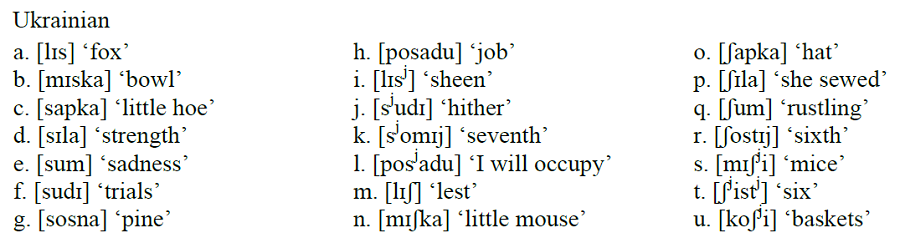
\includegraphics{../images/ukrainian.png}
\end{figure}

~\\
INSTRUCTOR NOTES: 


\vfill
Excellent (3) ~~~ Good (2.2) ~~~ Fair (1.7) ~~~ Poor (0)
\newpage

{\large Question 2}\\

Source: Day 2 Discussion\\

Assuming a Standard North American English inventory, does this vowel need to have tenseness specified if you're giving a prose description? Why or why not?\\

{[u]}


~\\
INSTRUCTOR NOTES: yes


\vfill
Excellent (3) ~~~ Good (2.2) ~~~ Fair (1.7) ~~~ Poor (0)
\newpage

{\large Question 3}\\

Source: Day 2 Handout, Part I, Question 11\\

How would this word be transcribed?\\ Follow-up question: Why did you use symbol [X] instead of symbol [Y]?\\

<square>


~\\
INSTRUCTOR NOTES: [skweɪɹ]


\vfill
Excellent (3) ~~~ Good (2.2) ~~~ Fair (1.7) ~~~ Poor (0)
\newpage

{\large Question 4}\\

Source: Day 6 Handout, Question 11\\

What do the two signs below tell you about the phonological status of \underline{handshape} in ASL, and why?\\

\begin{figure}[H]
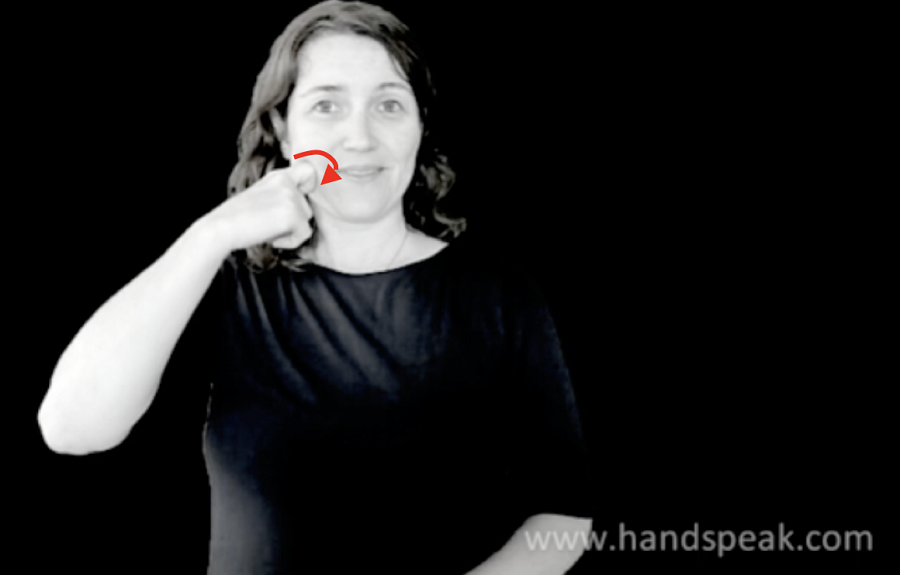
\includegraphics{../images/asl_apple.png}
\caption{APPLE}
\end{figure}
\begin{figure}[H]
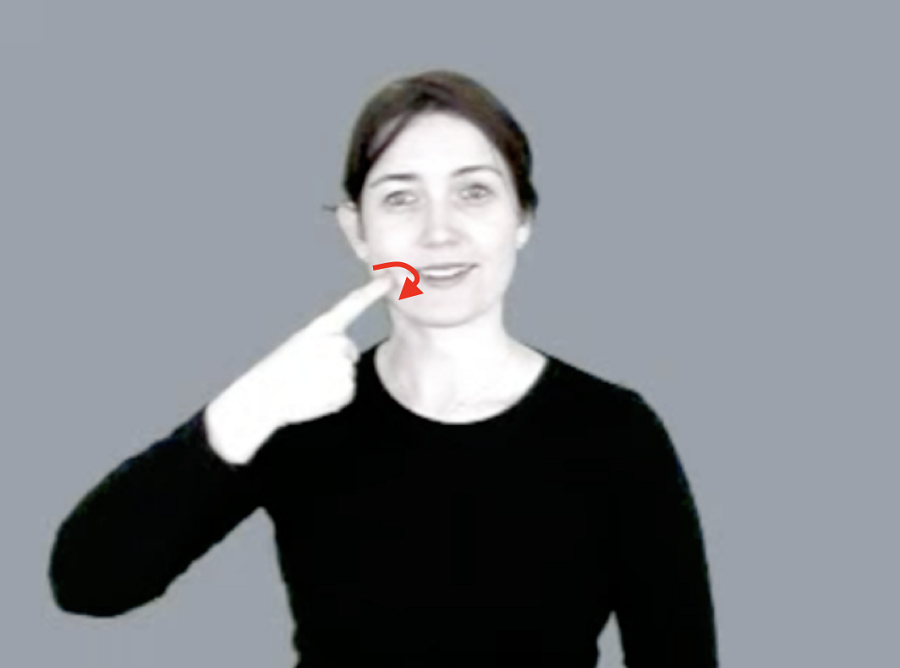
\includegraphics{../images/asl_candy.png}
\caption{CANDY}
\end{figure}

~\\
INSTRUCTOR NOTES: shows contrast because movement and location are same


\vfill
Excellent (3) ~~~ Good (2.2) ~~~ Fair (1.7) ~~~ Poor (0)
\newpage

{\large Question 5}\\

Source: Day 7 Handout, Question 2\\

Explain whether the rule below would apply to the form shown, and if so, what the effect of the rule would be. Assume the vowel inventory [i], [ɪ], [e], [ɛ], [ɑ], [u], [ʊ], [o], [ɔ].\\

/emos/

{[non-low vowel]} →  {[lax]} / \_\_ C$_0$ {[lax vowel]}


~\\
INSTRUCTOR NOTES: doesn't apply


\vfill
Excellent (3) ~~~ Good (2.2) ~~~ Fair (1.7) ~~~ Poor (0)
\newpage

\begin{center}
\textbf{{\color{red}{\HUGE END OF EXAM}}}\\

\end{center}
\newpage

\begin{center}
\textbf{{\color{blue}{\HUGE START OF EXAM\\}}}

\textbf{{\color{blue}{\HUGE Student ID: 3129\\}}}

\textbf{{\color{blue}{\HUGE 12:00 noon - 12:15 PM\\}}}

\end{center}
\newpage

{\large Question 1}\\

Source: Quiz 3, Question 1\\

L$_X$ (Language X) has three vowels, [i], [a], and [u]. It has bi-syllabic roots like Kikuyu. It does not allow non-identical high vowels to co-occur. Of the following nine logically possible vocalic sequences, which ones should be unattested in L$_X$? Explain why.\\

\begin{itemize} \item {[i...i]} \item {[i...a]} \item {[i...u]} \item {[a...i]} \item {[a...a]} \item {[a...u]} \item {[u...i]} \item {[u...a]} \item {[u...u]} \end{itemize}


~\\
INSTRUCTOR NOTES: [i...u], [u...i]


\vfill
Excellent (3) ~~~ Good (2.2) ~~~ Fair (1.7) ~~~ Poor (0)
\newpage

{\large Question 2}\\

Source: Homework 1, Question 3(b)\\

Explain why this is or is not a complete natural class in standard North American English.\\

{[ɔ]}, {[ʊ]}, {[u]}, {[oʊ]}


~\\
INSTRUCTOR NOTES: yes (all back rounded vowels)


\vfill
Excellent (3) ~~~ Good (2.2) ~~~ Fair (1.7) ~~~ Poor (0)
\newpage

{\large Question 3}\\

Source: Day 7 Handout, Question 11\\

What is the basic analysis of voiceless stops in this dataset, and what are the key pieces of evidence?\\

\begin{figure}[H]
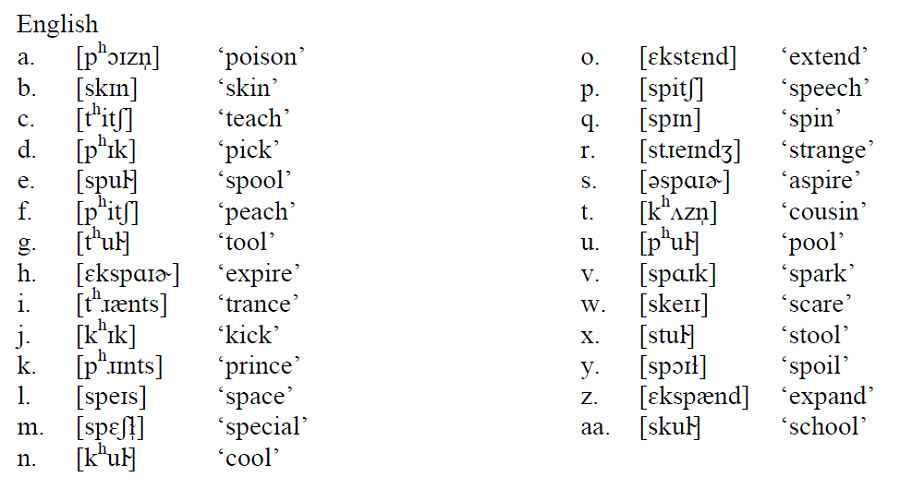
\includegraphics{../images/english11.png}
\end{figure}

~\\
INSTRUCTOR NOTES: Plain and aspirated voiceless stops are in complementary distribution in English. Plain stops occur always and only after [s], as in [speɪs] ‘space,’ while aspirated stops never occur in this context. Meanwhile, aspirated stops occur word-initially (e.g., [phitʃ] ‘peach’) and between vowels (e.g., [əphɑɹt] ‘apart’). Because the two are in complementary distribution, we can always predict which one occurs in any given environment, and so we conclude that they are allophonic, i.e., allophones of the same phoneme category. 


\vfill
Excellent (3) ~~~ Good (2.2) ~~~ Fair (1.7) ~~~ Poor (0)
\newpage

{\large Question 4}\\

Source: Day 2 Handout, Part I, Question 11\\

How would this word be transcribed?\\ Follow-up question: Why did you use symbol [X] instead of symbol [Y]?\\

<juice>


~\\
INSTRUCTOR NOTES: [dʒus]


\vfill
Excellent (3) ~~~ Good (2.2) ~~~ Fair (1.7) ~~~ Poor (0)
\newpage

{\large Question 5}\\

Source: Day 2 Discussion\\

Assuming a Standard North American English inventory, does this vowel need to have tenseness specified if you're giving a prose description? Why or why not?\\

{[u]}


~\\
INSTRUCTOR NOTES: yes


\vfill
Excellent (3) ~~~ Good (2.2) ~~~ Fair (1.7) ~~~ Poor (0)
\newpage

\begin{center}
\textbf{{\color{red}{\HUGE END OF EXAM}}}\\

\end{center}
\newpage

\begin{center}
\textbf{{\color{blue}{\HUGE START OF EXAM\\}}}

\textbf{{\color{blue}{\HUGE Student ID: 7661\\}}}

\textbf{{\color{blue}{\HUGE 12:15 PM - 12:30 PM\\}}}

\end{center}
\newpage

{\large Question 1}\\

Source: Quiz 3, Question 1\\

L$_X$ (Language X) has three vowels, [i], [a], and [u]. It has bi-syllabic roots like Kikuyu. It does not allow non-identical high vowels to co-occur. Of the following nine logically possible vocalic sequences, which ones should be unattested in L$_X$? Explain why.\\

\begin{itemize} \item {[i...i]} \item {[i...a]} \item {[i...u]} \item {[a...i]} \item {[a...a]} \item {[a...u]} \item {[u...i]} \item {[u...a]} \item {[u...u]} \end{itemize}


~\\
INSTRUCTOR NOTES: [i...u], [u...i]


\vfill
Excellent (3) ~~~ Good (2.2) ~~~ Fair (1.7) ~~~ Poor (0)
\newpage

{\large Question 2}\\

Source: Day 7 Handout, Question 9\\

What is the basic analysis of vowel length in this dataset, and what are the key pieces of evidence?\\

\begin{figure}[H]
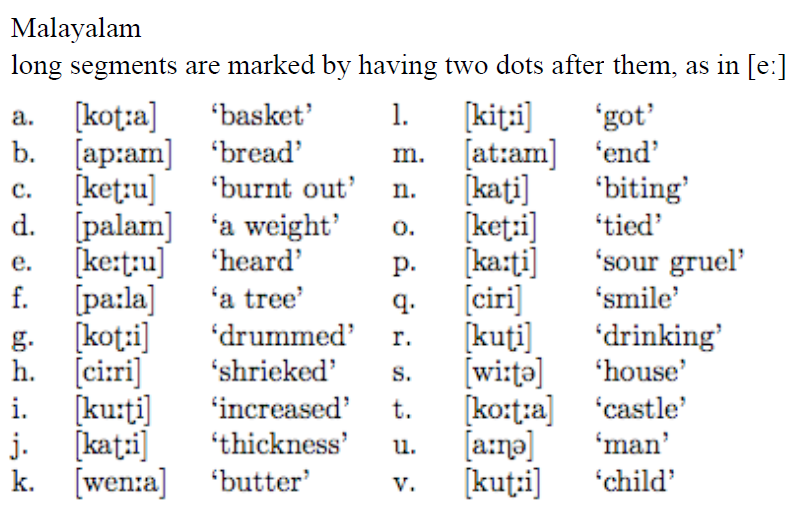
\includegraphics{../images/malayalam.png}
\end{figure}

~\\
INSTRUCTOR NOTES: Short and long vowels appear to be contrastive (phonemic) in Malayalam, as evidenced by minimal pairs that differ only in terms of their vowel length, such as [koʈːa] ‘basket’ vs. [koːʈːa] ‘castle’ or [keʈːu] ‘burnt out’ vs. [keːʈːu] ‘heard.’


\vfill
Excellent (3) ~~~ Good (2.2) ~~~ Fair (1.7) ~~~ Poor (0)
\newpage

{\large Question 3}\\

Source: Day 6 Handout, Question 7\\

Explain how you would determine the phonological relationship between these two sounds (given below) in this dataset.\\

{[s]} and {[z]}

\begin{figure}[H]
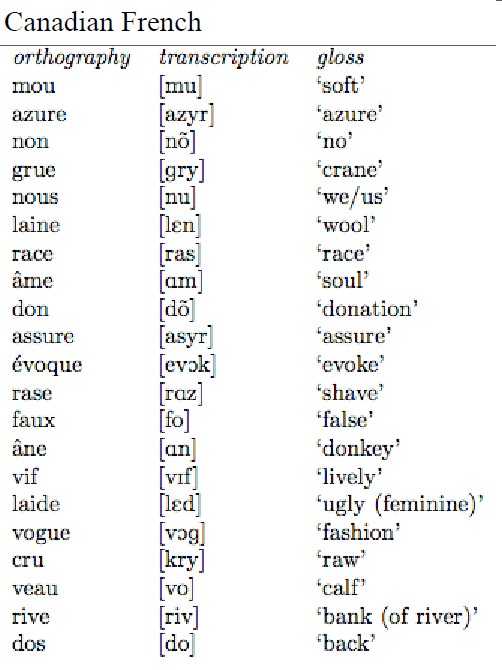
\includegraphics{../images/canadianfrench.png}
\end{figure}

~\\
INSTRUCTOR NOTES: contrastive; [asyr] ‘assure’ vs. [azyr] ‘azure’


\vfill
Excellent (3) ~~~ Good (2.2) ~~~ Fair (1.7) ~~~ Poor (0)
\newpage

{\large Question 4}\\

Source: Day 2 Discussion\\

Assuming a Standard North American English inventory, does this vowel need to have tenseness specified if you're giving a prose description? Why or why not?\\

{[ɑ]}


~\\
INSTRUCTOR NOTES: no


\vfill
Excellent (3) ~~~ Good (2.2) ~~~ Fair (1.7) ~~~ Poor (0)
\newpage

{\large Question 5}\\

Source: Day 2 Handout, Part I, Question 11\\

How would this word be transcribed?\\ Follow-up question: Why did you use symbol [X] instead of symbol [Y]?\\

<toy>


~\\
INSTRUCTOR NOTES: [tɔɪ]


\vfill
Excellent (3) ~~~ Good (2.2) ~~~ Fair (1.7) ~~~ Poor (0)
\newpage

\begin{center}
\textbf{{\color{red}{\HUGE END OF EXAM}}}\\

\end{center}
\newpage

\begin{center}
\textbf{{\color{blue}{\HUGE START OF EXAM\\}}}

\textbf{{\color{blue}{\HUGE Student ID: 3684\\}}}

\textbf{{\color{blue}{\HUGE 12:30 - 12:45 PM\\}}}

\end{center}
\newpage

{\large Question 1}\\

Source: Quiz 3, Question 2\\

L$_X$ has tri-syllabic roots. If L$_X$ does not allow non-identical high vowels to co-occur, which one of the following tri-syllabic vocalic sequences do you predict to be unattested in L$_X$? Explain why.\\

\begin{itemize} \item {[u...i...a]} \item {[a...i...a]} \item {[u...u...a]} \item {[a...i...i]} \end{itemize}


~\\
INSTRUCTOR NOTES: [u...i...a]


\vfill
Excellent (3) ~~~ Good (2.2) ~~~ Fair (1.7) ~~~ Poor (0)
\newpage

{\large Question 2}\\

Source: Day 7 Handout, Question 11\\

What is the basic analysis of voiceless stops in this dataset, and what are the key pieces of evidence?\\

\begin{figure}[H]
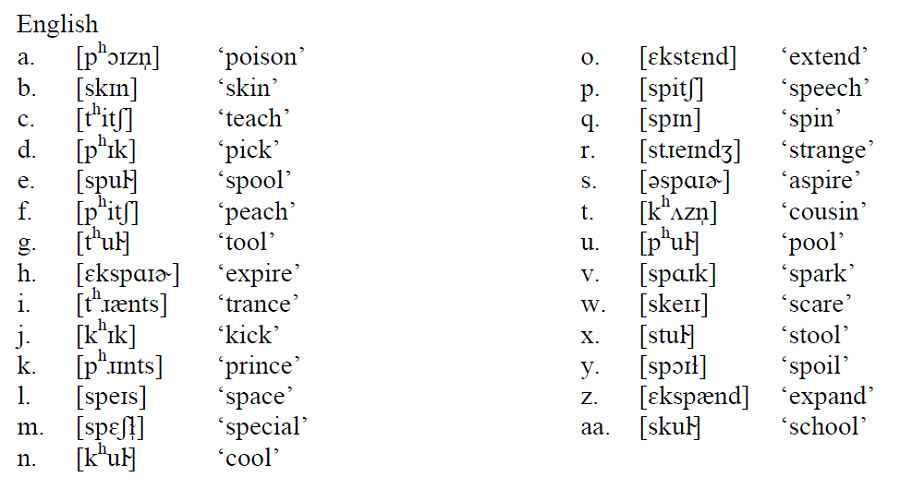
\includegraphics{../images/english11.png}
\end{figure}

~\\
INSTRUCTOR NOTES: Plain and aspirated voiceless stops are in complementary distribution in English. Plain stops occur always and only after [s], as in [speɪs] ‘space,’ while aspirated stops never occur in this context. Meanwhile, aspirated stops occur word-initially (e.g., [phitʃ] ‘peach’) and between vowels (e.g., [əphɑɹt] ‘apart’). Because the two are in complementary distribution, we can always predict which one occurs in any given environment, and so we conclude that they are allophonic, i.e., allophones of the same phoneme category. 


\vfill
Excellent (3) ~~~ Good (2.2) ~~~ Fair (1.7) ~~~ Poor (0)
\newpage

{\large Question 3}\\

Source: Homework 1, Question 3(b)\\

Explain why this is or is not a complete natural class in standard North American English.\\

{[b]}, {[n]}, {[ɡ]}, {[ʒ]}, {[v]}


~\\
INSTRUCTOR NOTES: no; lots of other voiced consonants


\vfill
Excellent (3) ~~~ Good (2.2) ~~~ Fair (1.7) ~~~ Poor (0)
\newpage

{\large Question 4}\\

Source: Day 2 Handout, Part I, Question 11\\

How would this word be transcribed?\\ Follow-up question: Why did you use symbol [X] instead of symbol [Y]?\\

<bird>


~\\
INSTRUCTOR NOTES: [bɹ̩d]


\vfill
Excellent (3) ~~~ Good (2.2) ~~~ Fair (1.7) ~~~ Poor (0)
\newpage

{\large Question 5}\\

Source: Day 2 Handout, Part I, Question 11\\

How would this word be transcribed?\\ Follow-up question: Why did you use symbol [X] instead of symbol [Y]?\\

<segment>


~\\
INSTRUCTOR NOTES: [sɛɡmɛnt]


\vfill
Excellent (3) ~~~ Good (2.2) ~~~ Fair (1.7) ~~~ Poor (0)
\newpage

\begin{center}
\textbf{{\color{red}{\HUGE END OF EXAM}}}\\

\end{center}
\newpage

\begin{center}
\textbf{{\color{blue}{\HUGE START OF EXAM\\}}}

\textbf{{\color{blue}{\HUGE Student ID: 3737\\}}}

\textbf{{\color{blue}{\HUGE 12:45 - 1:00 PM\\}}}

\end{center}
\newpage

{\large Question 1}\\

Source: Day 5 Handout, Question 5\\

How would you look for co-occurrence restrictions between [s] and the vowels that come after it in this dataset?\\

\begin{figure}[H]
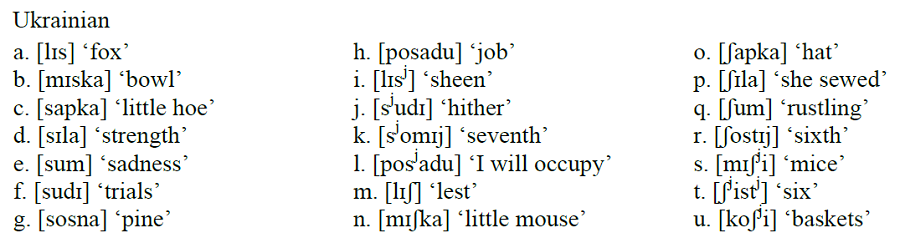
\includegraphics{../images/ukrainian.png}
\end{figure}

~\\
INSTRUCTOR NOTES: 


\vfill
Excellent (3) ~~~ Good (2.2) ~~~ Fair (1.7) ~~~ Poor (0)
\newpage

{\large Question 2}\\

Source: Day 7 Handout, Question 12\\

What is the basic analysis of oral and nasal vowels in this dataset, and what are the key pieces of evidence?\\

\begin{figure}[H]
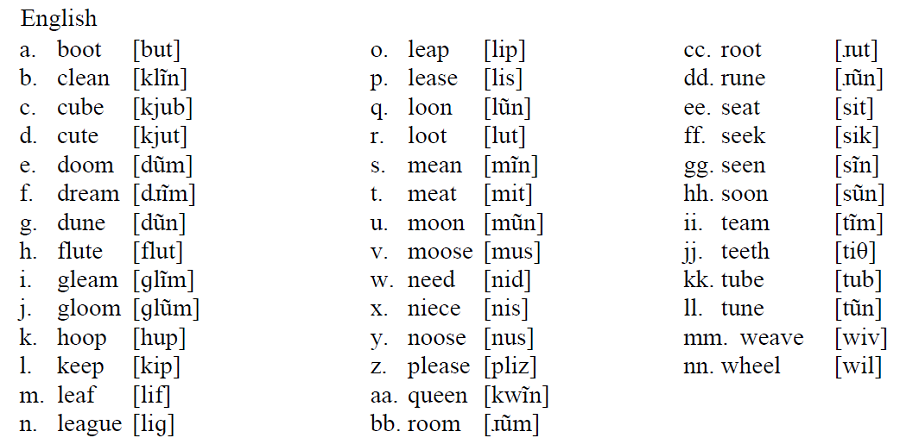
\includegraphics{../images/english12.png}
\end{figure}

~\\
INSTRUCTOR NOTES: The pairs of sounds [i] and [ĩ], and [u] and [ũ], are each allophonic and therefore allophones of the same phoneme in English (though the two pairs represent two contrastive phonemes in English). The sounds [i] and [ĩ] are in complementary distribution in English, with [ĩ] occurring before the sounds [m] and [n], (e.g., [ɡlĩm] ‘gleam’ and [klĩn] ‘clean’) and [i] occurring elsewhere (e.g., [lip] ‘leap’). Similarly, the sounds [u] and [ũ] are also in complementary distribution, with exactly the same conditioning environments: [ũ] occurs before [m] and [n] (e.g., [dũm] ‘doom’ and [dũn] ‘dune’), and [u] occurs elsewhere (e.g. [but] ‘boot’). Thus, within each pair, we treat the vowels as allophonic. 


\vfill
Excellent (3) ~~~ Good (2.2) ~~~ Fair (1.7) ~~~ Poor (0)
\newpage

{\large Question 3}\\

Source: Day 2 Handout, Part I, Question 11\\

How would this word be transcribed?\\ Follow-up question: Why did you use symbol [X] instead of symbol [Y]?\\

<bird>


~\\
INSTRUCTOR NOTES: [bɹ̩d]


\vfill
Excellent (3) ~~~ Good (2.2) ~~~ Fair (1.7) ~~~ Poor (0)
\newpage

{\large Question 4}\\

Source: Day 4 Handout, Question 2(iv)\\

Explain how you would figure out the Swahili word for this English gloss.\\

‘I wanted them.’

\begin{figure}[H]
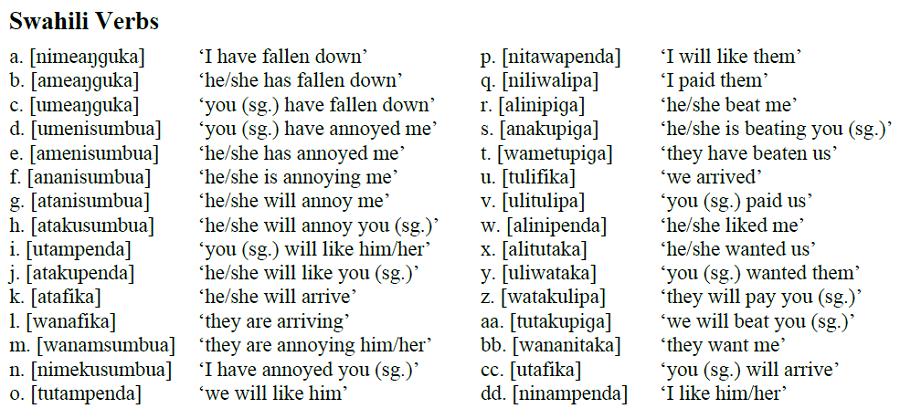
\includegraphics{../images/swahiliverbs.png}
\end{figure}

~\\
INSTRUCTOR NOTES: ([niliwataka])


\vfill
Excellent (3) ~~~ Good (2.2) ~~~ Fair (1.7) ~~~ Poor (0)
\newpage

{\large Question 5}\\

Source: Day 2 Handout, Part II, Question 13\\

Explain why this image does or does not match the description.\\

\begin{itemize} \item A one-handed sign. \item Location: In front of signer’s chin. \item Handshape: Starts with an “L” shape; proximal joint of index finger folds down during the sign. \item Movement: Hand starts on far side of signer’s body and moves horizontally straight across. \end{itemize}

\begin{figure}[H]
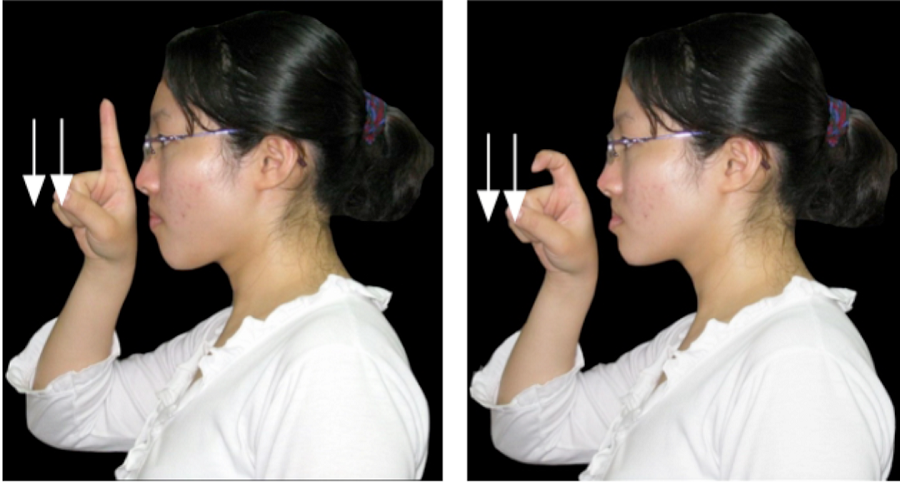
\includegraphics{../images/taiwansign_jealous.png}
\caption{JEALOUS}
\end{figure}

~\\
INSTRUCTOR NOTES: no; handshape and movement are wrong


\vfill
Excellent (3) ~~~ Good (2.2) ~~~ Fair (1.7) ~~~ Poor (0)
\newpage

\begin{center}
\textbf{{\color{red}{\HUGE END OF EXAM}}}\\

\end{center}
\newpage

\begin{center}
\textbf{{\color{blue}{\HUGE START OF EXAM\\}}}

\textbf{{\color{blue}{\HUGE Student ID: 5824\\}}}

\textbf{{\color{blue}{\HUGE 1:00 - 1:15 PM\\}}}

\end{center}
\newpage

{\large Question 1}\\

Source: Day 5 Handout, Question 3\\

What evidence is there that there is a pattern in these data, assuming that these are the only CV and VC sequences that occur in some language?\\

{[sa]}, {[ʃi]}, {[za]}, {[ʒi]}, {[as]}, {[iʃ]}, {[az]}, {[iʒ]}


~\\
INSTRUCTOR NOTES: (the palatal sounds occur with the high vowel, while the alveolar sounds occur with the low vowel)


\vfill
Excellent (3) ~~~ Good (2.2) ~~~ Fair (1.7) ~~~ Poor (0)
\newpage

{\large Question 2}\\

Source: Day 2 Handout, Part I, Question 11\\

How would this word be transcribed?\\ Follow-up question: Why did you use symbol [X] instead of symbol [Y]?\\

<finger>


~\\
INSTRUCTOR NOTES: [fɪŋɡɹ̩]


\vfill
Excellent (3) ~~~ Good (2.2) ~~~ Fair (1.7) ~~~ Poor (0)
\newpage

{\large Question 3}\\

Source: Quiz 2, Question 6\\

In the pronunciation of this word, which sounds are obstruents and which are sonorants?\\

<sonorant>


~\\
INSTRUCTOR NOTES: [sɔnoɹənt] -- sonorants: [ɔnoɹən] and obstruents: [st]


\vfill
Excellent (3) ~~~ Good (2.2) ~~~ Fair (1.7) ~~~ Poor (0)
\newpage

{\large Question 4}\\

Source: Day 2 Handout, Part I, Question 11\\

How would this word be transcribed?\\ Follow-up question: Why did you use symbol [X] instead of symbol [Y]?\\

<toy>


~\\
INSTRUCTOR NOTES: [tɔɪ]


\vfill
Excellent (3) ~~~ Good (2.2) ~~~ Fair (1.7) ~~~ Poor (0)
\newpage

{\large Question 5}\\

Source: Day 6 Handout, Question 11\\

What do the two signs below tell you about the phonological status of \underline{handshape} in ASL, and why?\\

\begin{figure}[H]
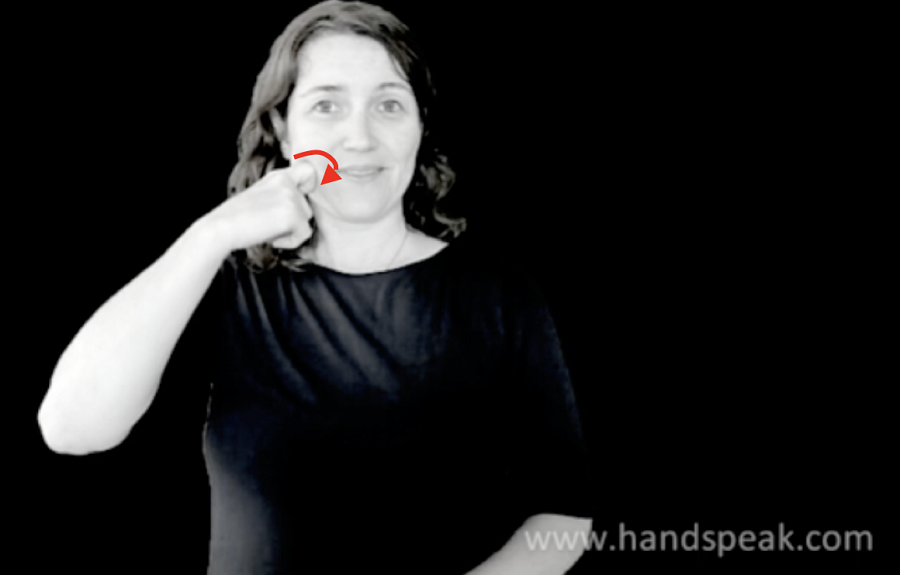
\includegraphics{../images/asl_apple.png}
\caption{APPLE}
\end{figure}
\begin{figure}[H]
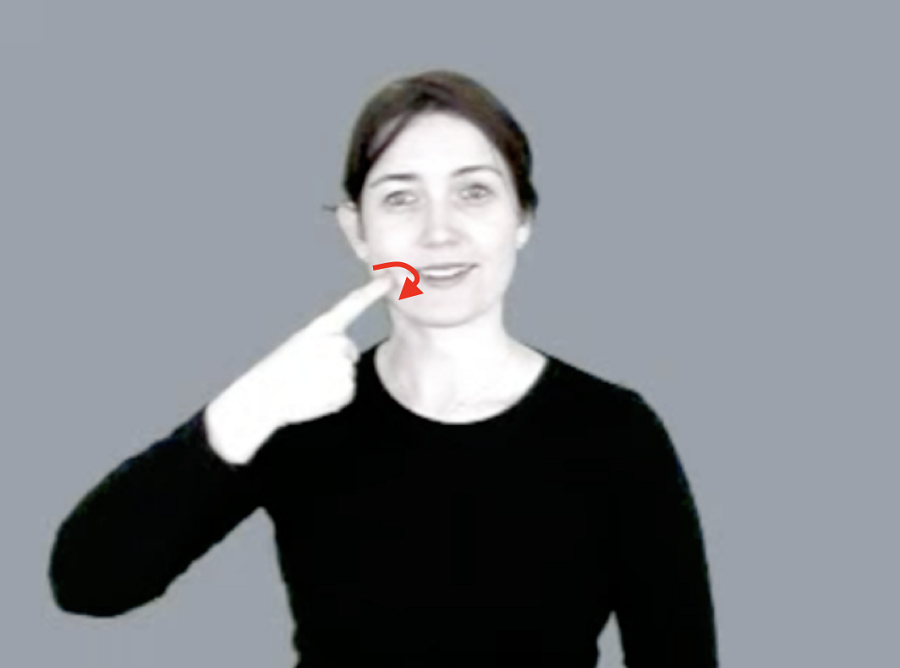
\includegraphics{../images/asl_candy.png}
\caption{CANDY}
\end{figure}

~\\
INSTRUCTOR NOTES: shows contrast because movement and location are same


\vfill
Excellent (3) ~~~ Good (2.2) ~~~ Fair (1.7) ~~~ Poor (0)
\newpage

\begin{center}
\textbf{{\color{red}{\HUGE END OF EXAM}}}\\

\end{center}
\newpage

\begin{center}
\textbf{{\color{blue}{\HUGE START OF EXAM\\}}}

\textbf{{\color{blue}{\HUGE Student ID: 1743\\}}}

\textbf{{\color{blue}{\HUGE 1:15 - 1:30 PM\\}}}

\end{center}
\newpage

{\large Question 1}\\

Source: Day 5 Handout, Question 3\\

What evidence is there that there is a pattern in these data, assuming that these are the only CV and VC sequences that occur in some language?\\

{[sa]}, {[ʃi]}, {[za]}, {[ʒi]}, {[as]}, {[iʃ]}, {[az]}, {[iʒ]}


~\\
INSTRUCTOR NOTES: (the palatal sounds occur with the high vowel, while the alveolar sounds occur with the low vowel)


\vfill
Excellent (3) ~~~ Good (2.2) ~~~ Fair (1.7) ~~~ Poor (0)
\newpage

{\large Question 2}\\

Source: Day 2 Handout, Part I, Question 11\\

How would this word be transcribed?\\ Follow-up question: Why did you use symbol [X] instead of symbol [Y]?\\

<toy>


~\\
INSTRUCTOR NOTES: [tɔɪ]


\vfill
Excellent (3) ~~~ Good (2.2) ~~~ Fair (1.7) ~~~ Poor (0)
\newpage

{\large Question 3}\\

Source: Day 2 Discussion\\

Assuming a Standard North American English inventory, does this vowel need to have tenseness specified if you're giving a prose description? Why or why not?\\

{[æ]}


~\\
INSTRUCTOR NOTES: no


\vfill
Excellent (3) ~~~ Good (2.2) ~~~ Fair (1.7) ~~~ Poor (0)
\newpage

{\large Question 4}\\

Source: Day 6 Handout, Question 11\\

What do the two signs below tell you about the phonological status of \underline{handshape} in ASL, and why?\\

\begin{figure}[H]
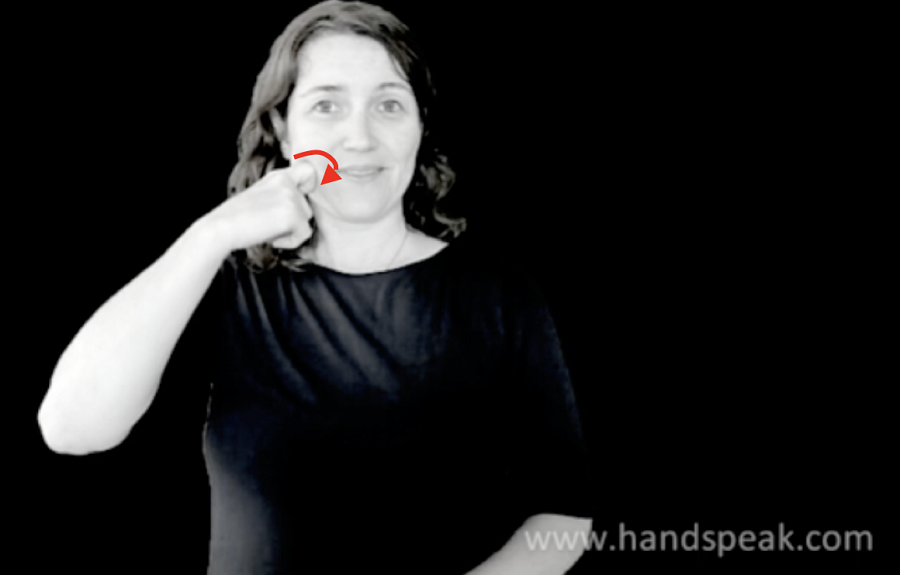
\includegraphics{../images/asl_apple.png}
\caption{APPLE}
\end{figure}
\begin{figure}[H]
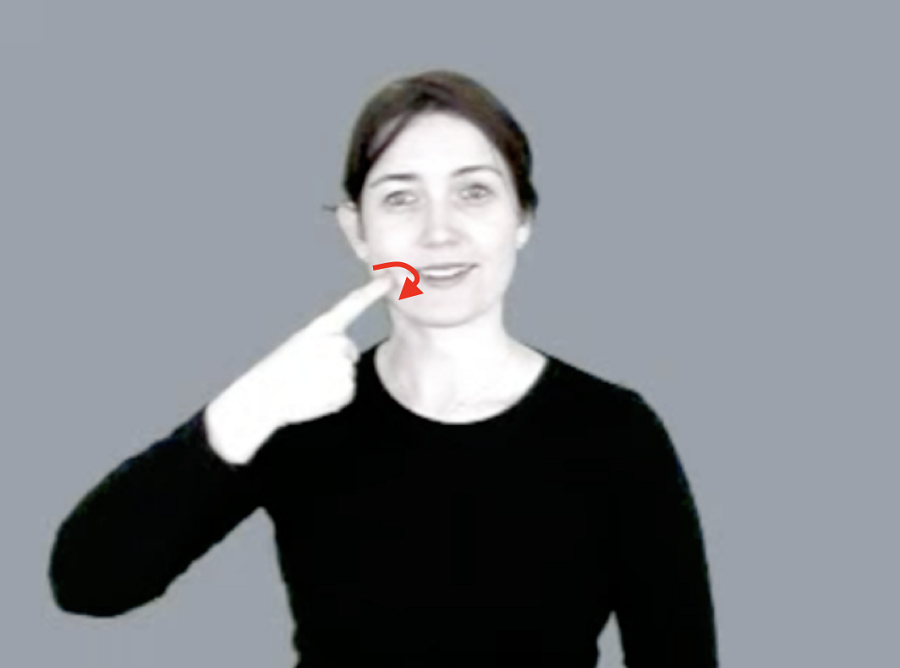
\includegraphics{../images/asl_candy.png}
\caption{CANDY}
\end{figure}

~\\
INSTRUCTOR NOTES: shows contrast because movement and location are same


\vfill
Excellent (3) ~~~ Good (2.2) ~~~ Fair (1.7) ~~~ Poor (0)
\newpage

{\large Question 5}\\

Source: Day 2 Discussion\\

Assuming a Standard North American English inventory, does this vowel need to have tenseness specified if you're giving a prose description? Why or why not?\\

{[u]}


~\\
INSTRUCTOR NOTES: yes


\vfill
Excellent (3) ~~~ Good (2.2) ~~~ Fair (1.7) ~~~ Poor (0)
\newpage

\begin{center}
\textbf{{\color{red}{\HUGE END OF EXAM}}}\\

\end{center}
\newpage

\begin{center}
\textbf{{\color{blue}{\HUGE START OF EXAM\\}}}

\textbf{{\color{blue}{\HUGE Student ID: 2014\\}}}

\textbf{{\color{blue}{\HUGE 1:30 - 1:45 PM\\}}}

\end{center}
\newpage

{\large Question 1}\\

Source: Day 5 Handout, Question 3\\

What evidence is there that there is a pattern in these data, assuming that these are the only CV and VC sequences that occur in some language?\\

{[sa]}, {[ʃi]}, {[za]}, {[ʒi]}, {[as]}, {[iʃ]}, {[az]}, {[iʒ]}


~\\
INSTRUCTOR NOTES: (the palatal sounds occur with the high vowel, while the alveolar sounds occur with the low vowel)


\vfill
Excellent (3) ~~~ Good (2.2) ~~~ Fair (1.7) ~~~ Poor (0)
\newpage

{\large Question 2}\\

Source: Homework 2, Question 2\\

Why should the following two questions have the same answer?\\

\begin{itemize} \item Given the vowel system of Jita, how many bi-syllabic root types would you expect to find for nouns in the language? \item Assuming that the vowel inventory is the same in verbs as it is in nouns, how many bisyllabic root types would you expect to find for verbs in the language? \end{itemize}


~\\
INSTRUCTOR NOTES: 


\vfill
Excellent (3) ~~~ Good (2.2) ~~~ Fair (1.7) ~~~ Poor (0)
\newpage

{\large Question 3}\\

Source: Day 2 Handout, Part I, Question 11\\

How would this word be transcribed?\\ Follow-up question: Why did you use symbol [X] instead of symbol [Y]?\\

<nice>


~\\
INSTRUCTOR NOTES: [nɑɪs]


\vfill
Excellent (3) ~~~ Good (2.2) ~~~ Fair (1.7) ~~~ Poor (0)
\newpage

{\large Question 4}\\

Source: Quiz 2, Question 6\\

In the pronunciation of this word, which sounds are obstruents and which are sonorants?\\

<minimal>


~\\
INSTRUCTOR NOTES: [mɪnɪməl] -- sonorants: (all of them)


\vfill
Excellent (3) ~~~ Good (2.2) ~~~ Fair (1.7) ~~~ Poor (0)
\newpage

{\large Question 5}\\

Source: Day 7 Handout, Question 9\\

What is the basic analysis of vowel length in this dataset, and what are the key pieces of evidence?\\

\begin{figure}[H]
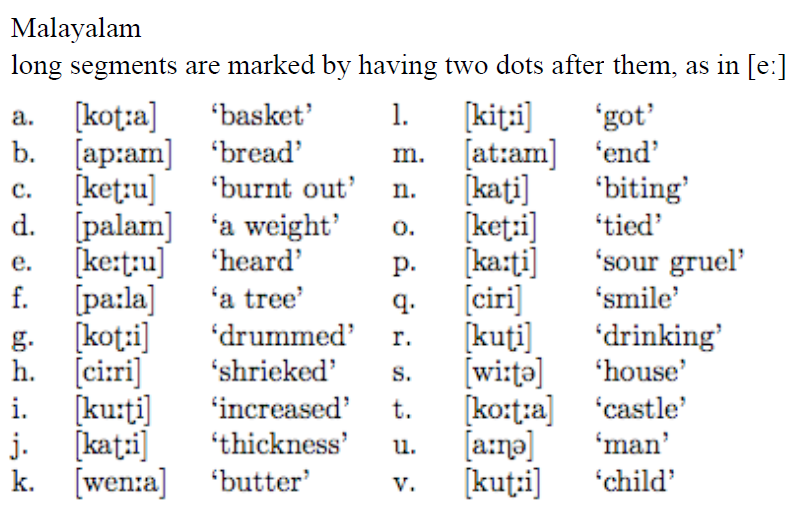
\includegraphics{../images/malayalam.png}
\end{figure}

~\\
INSTRUCTOR NOTES: Short and long vowels appear to be contrastive (phonemic) in Malayalam, as evidenced by minimal pairs that differ only in terms of their vowel length, such as [koʈːa] ‘basket’ vs. [koːʈːa] ‘castle’ or [keʈːu] ‘burnt out’ vs. [keːʈːu] ‘heard.’


\vfill
Excellent (3) ~~~ Good (2.2) ~~~ Fair (1.7) ~~~ Poor (0)
\newpage

\begin{center}
\textbf{{\color{red}{\HUGE END OF EXAM}}}\\

\end{center}
\newpage

\begin{center}
\textbf{{\color{blue}{\HUGE START OF EXAM\\}}}

\textbf{{\color{blue}{\HUGE Student ID: 9657\\}}}

\textbf{{\color{blue}{\HUGE 1:45 - 2:00 PM\\}}}

\end{center}
\newpage

{\large Question 1}\\

Source: Quiz 3, Question 1\\

L$_X$ (Language X) has three vowels, [i], [a], and [u]. It has bi-syllabic roots like Kikuyu. It does not allow non-identical high vowels to co-occur. Of the following nine logically possible vocalic sequences, which ones should be unattested in L$_X$? Explain why.\\

\begin{itemize} \item {[i...i]} \item {[i...a]} \item {[i...u]} \item {[a...i]} \item {[a...a]} \item {[a...u]} \item {[u...i]} \item {[u...a]} \item {[u...u]} \end{itemize}


~\\
INSTRUCTOR NOTES: [i...u], [u...i]


\vfill
Excellent (3) ~~~ Good (2.2) ~~~ Fair (1.7) ~~~ Poor (0)
\newpage

{\large Question 2}\\

Source: Day 2 Handout, Part I, Question 11\\

How would this word be transcribed?\\ Follow-up question: Why did you use symbol [X] instead of symbol [Y]?\\

<goat>


~\\
INSTRUCTOR NOTES: [ɡoʊt]


\vfill
Excellent (3) ~~~ Good (2.2) ~~~ Fair (1.7) ~~~ Poor (0)
\newpage

{\large Question 3}\\

Source: Day 4 Handout, Question 2(iv)\\

Explain how you would figure out the Swahili word for this English gloss.\\

‘I like you (sg.).’

\begin{figure}[H]
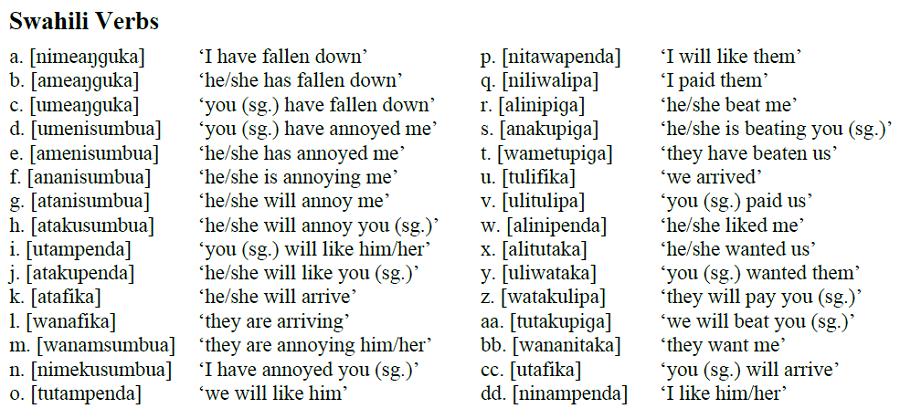
\includegraphics{../images/swahiliverbs.png}
\end{figure}

~\\
INSTRUCTOR NOTES: ([ninakupenda])


\vfill
Excellent (3) ~~~ Good (2.2) ~~~ Fair (1.7) ~~~ Poor (0)
\newpage

{\large Question 4}\\

Source: Day 7 Handout, Question 9\\

What is the basic analysis of vowel length in this dataset, and what are the key pieces of evidence?\\

\begin{figure}[H]
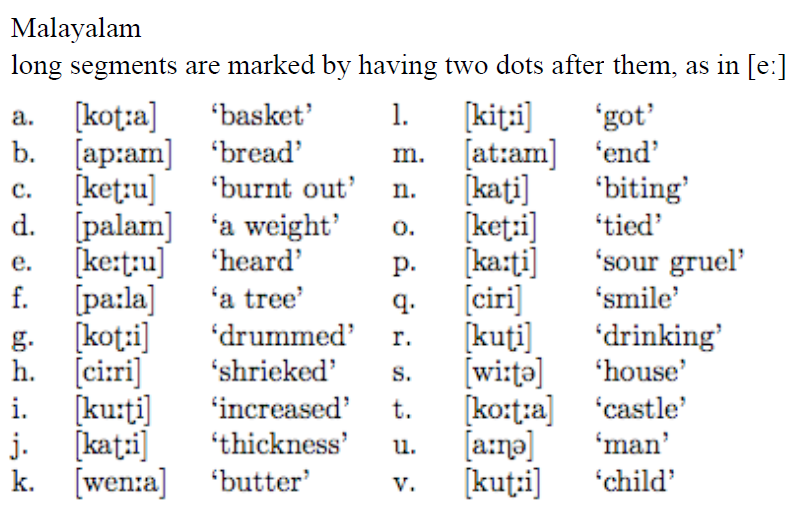
\includegraphics{../images/malayalam.png}
\end{figure}

~\\
INSTRUCTOR NOTES: Short and long vowels appear to be contrastive (phonemic) in Malayalam, as evidenced by minimal pairs that differ only in terms of their vowel length, such as [koʈːa] ‘basket’ vs. [koːʈːa] ‘castle’ or [keʈːu] ‘burnt out’ vs. [keːʈːu] ‘heard.’


\vfill
Excellent (3) ~~~ Good (2.2) ~~~ Fair (1.7) ~~~ Poor (0)
\newpage

{\large Question 5}\\

Source: Quiz 2, Question 6\\

In the pronunciation of this word, which sounds are obstruents and which are sonorants?\\

<obstruent>


~\\
INSTRUCTOR NOTES: [ɑbstɹuənt] -- sonorants: [ɑɹuən] and obstruents: [bstt]


\vfill
Excellent (3) ~~~ Good (2.2) ~~~ Fair (1.7) ~~~ Poor (0)
\newpage

\begin{center}
\textbf{{\color{red}{\HUGE END OF EXAM}}}\\

\end{center}
\newpage

\begin{center}
\textbf{{\color{blue}{\HUGE START OF EXAM\\}}}

\textbf{{\color{blue}{\HUGE Student ID: 9246\\}}}

\textbf{{\color{blue}{\HUGE 2:00 - 2:15 PM\\}}}

\end{center}
\newpage

{\large Question 1}\\

Source: Quiz 3, Question 1\\

L$_X$ (Language X) has three vowels, [i], [a], and [u]. It has bi-syllabic roots like Kikuyu. It does not allow non-identical high vowels to co-occur. Of the following nine logically possible vocalic sequences, which ones should be unattested in L$_X$? Explain why.\\

\begin{itemize} \item {[i...i]} \item {[i...a]} \item {[i...u]} \item {[a...i]} \item {[a...a]} \item {[a...u]} \item {[u...i]} \item {[u...a]} \item {[u...u]} \end{itemize}


~\\
INSTRUCTOR NOTES: [i...u], [u...i]


\vfill
Excellent (3) ~~~ Good (2.2) ~~~ Fair (1.7) ~~~ Poor (0)
\newpage

{\large Question 2}\\

Source: Day 7 Handout, Question 12\\

What is the basic analysis of oral and nasal vowels in this dataset, and what are the key pieces of evidence?\\

\begin{figure}[H]
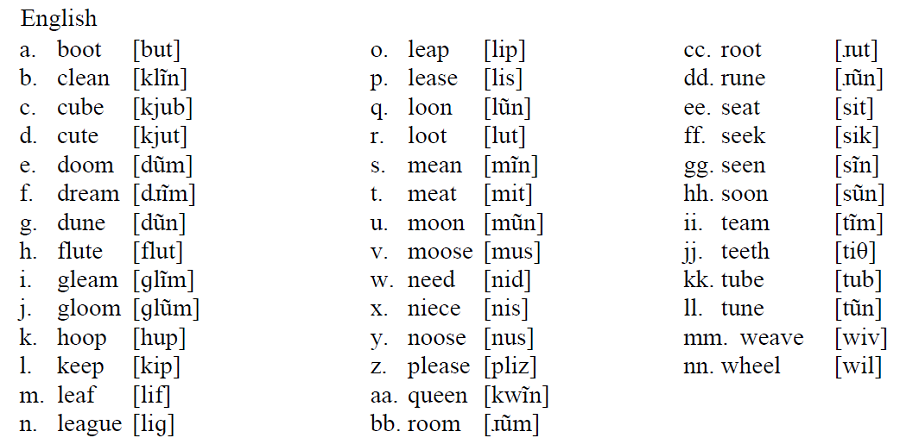
\includegraphics{../images/english12.png}
\end{figure}

~\\
INSTRUCTOR NOTES: The pairs of sounds [i] and [ĩ], and [u] and [ũ], are each allophonic and therefore allophones of the same phoneme in English (though the two pairs represent two contrastive phonemes in English). The sounds [i] and [ĩ] are in complementary distribution in English, with [ĩ] occurring before the sounds [m] and [n], (e.g., [ɡlĩm] ‘gleam’ and [klĩn] ‘clean’) and [i] occurring elsewhere (e.g., [lip] ‘leap’). Similarly, the sounds [u] and [ũ] are also in complementary distribution, with exactly the same conditioning environments: [ũ] occurs before [m] and [n] (e.g., [dũm] ‘doom’ and [dũn] ‘dune’), and [u] occurs elsewhere (e.g. [but] ‘boot’). Thus, within each pair, we treat the vowels as allophonic. 


\vfill
Excellent (3) ~~~ Good (2.2) ~~~ Fair (1.7) ~~~ Poor (0)
\newpage

{\large Question 3}\\

Source: Day 2 Handout, Part II, Question 7\\

Is the symbol given a reasonable way to transcribe any of the sounds described below? If so, which one? If not, why not?\\

{[n]}

\begin{itemize} \item voiceless palatal affricate \item voiced velar nasal \item voiceless glottal fricative \item voiced labiodental fricative \item voiced interdental fricative \item voiced palatal fricative \end{itemize}


~\\
INSTRUCTOR NOTES: no (voiced alveolar nasal)


\vfill
Excellent (3) ~~~ Good (2.2) ~~~ Fair (1.7) ~~~ Poor (0)
\newpage

{\large Question 4}\\

Source: Day 2 Handout, Part I, Question 11\\

How would this word be transcribed?\\ Follow-up question: Why did you use symbol [X] instead of symbol [Y]?\\

<goat>


~\\
INSTRUCTOR NOTES: [ɡoʊt]


\vfill
Excellent (3) ~~~ Good (2.2) ~~~ Fair (1.7) ~~~ Poor (0)
\newpage

{\large Question 5}\\

Source: Day 2 Handout, Part I, Question 11\\

How would this word be transcribed?\\ Follow-up question: Why did you use symbol [X] instead of symbol [Y]?\\

<little>


~\\
INSTRUCTOR NOTES: [lɪɾl̩]


\vfill
Excellent (3) ~~~ Good (2.2) ~~~ Fair (1.7) ~~~ Poor (0)
\newpage

\begin{center}
\textbf{{\color{red}{\HUGE END OF EXAM}}}\\

\end{center}
\newpage

\begin{center}
\textbf{{\color{blue}{\HUGE START OF EXAM\\}}}

\textbf{{\color{blue}{\HUGE Student ID: 4465\\}}}

\textbf{{\color{blue}{\HUGE 2:30 - 2:45 PM\\}}}

\end{center}
\newpage

{\large Question 1}\\

Source: Quiz 3, Question 1\\

L$_X$ (Language X) has three vowels, [i], [a], and [u]. It has bi-syllabic roots like Kikuyu. It does not allow non-identical high vowels to co-occur. Of the following nine logically possible vocalic sequences, which ones should be unattested in L$_X$? Explain why.\\

\begin{itemize} \item {[i...i]} \item {[i...a]} \item {[i...u]} \item {[a...i]} \item {[a...a]} \item {[a...u]} \item {[u...i]} \item {[u...a]} \item {[u...u]} \end{itemize}


~\\
INSTRUCTOR NOTES: [i...u], [u...i]


\vfill
Excellent (3) ~~~ Good (2.2) ~~~ Fair (1.7) ~~~ Poor (0)
\newpage

{\large Question 2}\\

Source: Day 2 Handout, Part I, Question 11\\

How would this word be transcribed?\\ Follow-up question: Why did you use symbol [X] instead of symbol [Y]?\\

<vacuum>


~\\
INSTRUCTOR NOTES: [vækjum]


\vfill
Excellent (3) ~~~ Good (2.2) ~~~ Fair (1.7) ~~~ Poor (0)
\newpage

{\large Question 3}\\

Source: Day 6 Handout, Question 11\\

What do the two signs below tell you about the phonological status of \underline{handshape} in ASL, and why?\\

\begin{figure}[H]
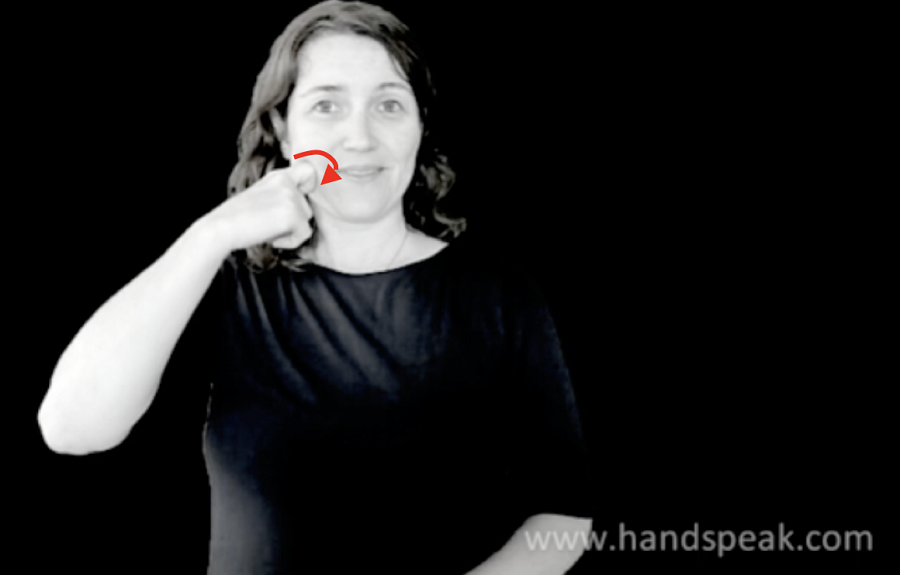
\includegraphics{../images/asl_apple.png}
\caption{APPLE}
\end{figure}
\begin{figure}[H]
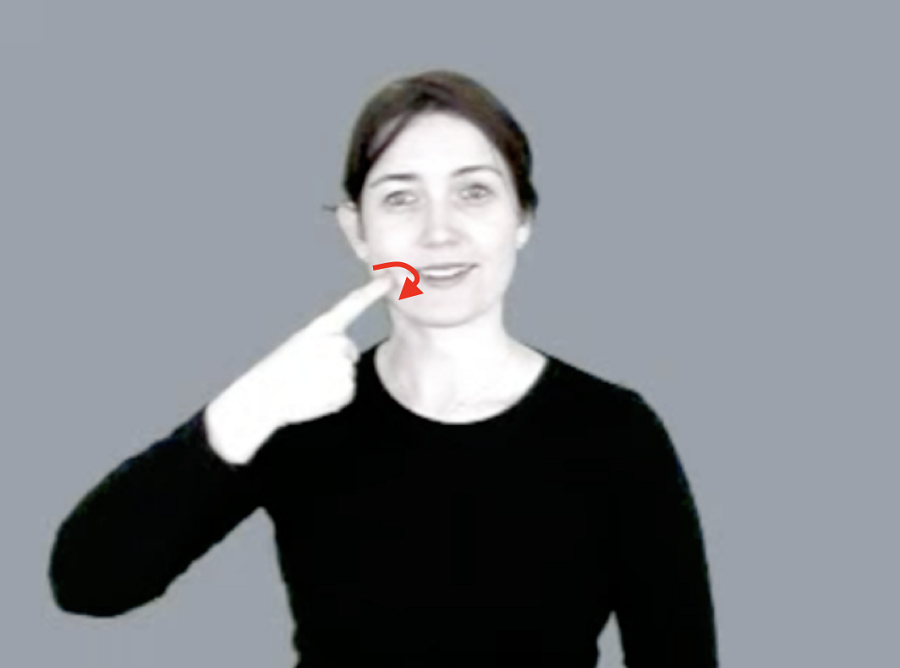
\includegraphics{../images/asl_candy.png}
\caption{CANDY}
\end{figure}

~\\
INSTRUCTOR NOTES: shows contrast because movement and location are same


\vfill
Excellent (3) ~~~ Good (2.2) ~~~ Fair (1.7) ~~~ Poor (0)
\newpage

{\large Question 4}\\

Source: Day 2 Handout, Part II, Question 7\\

Is the symbol given a reasonable way to transcribe any of the sounds described below? If so, which one? If not, why not?\\

{[ʃ]}

\begin{itemize} \item voiceless palatal affricate \item voiced velar nasal \item voiceless glottal fricative \item voiced labiodental fricative \item voiced interdental fricative \item voiced palatal fricative \end{itemize}


~\\
INSTRUCTOR NOTES: no (voiceless palatal fricative)


\vfill
Excellent (3) ~~~ Good (2.2) ~~~ Fair (1.7) ~~~ Poor (0)
\newpage

{\large Question 5}\\

Source: Day 6 Handout, Question 7\\

Explain how you would determine the phonological relationship between these two sounds (given below) in this dataset.\\

{[d]} and {[n]}

\begin{figure}[H]
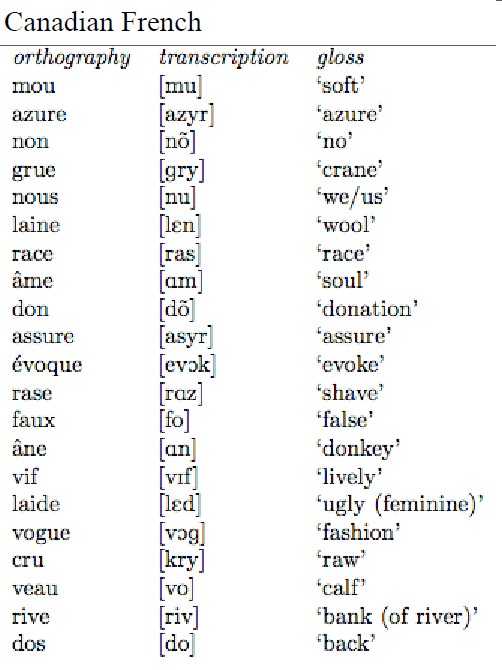
\includegraphics{../images/canadianfrench.png}
\end{figure}

~\\
INSTRUCTOR NOTES: contrastive; [do~] ‘donation’ vs. [no~] ‘no’


\vfill
Excellent (3) ~~~ Good (2.2) ~~~ Fair (1.7) ~~~ Poor (0)
\newpage

\begin{center}
\textbf{{\color{red}{\HUGE END OF EXAM}}}\\

\end{center}
\newpage

\begin{center}
\textbf{{\color{blue}{\HUGE START OF EXAM\\}}}

\textbf{{\color{blue}{\HUGE Student ID: 2931\\}}}

\textbf{{\color{blue}{\HUGE 2:45 - 3:00 PM\\}}}

\end{center}
\newpage

{\large Question 1}\\

Source: Day 5 Handout, Question 5\\

How would you look for co-occurrence restrictions between [s] and the vowels that come after it in this dataset?\\

\begin{figure}[H]
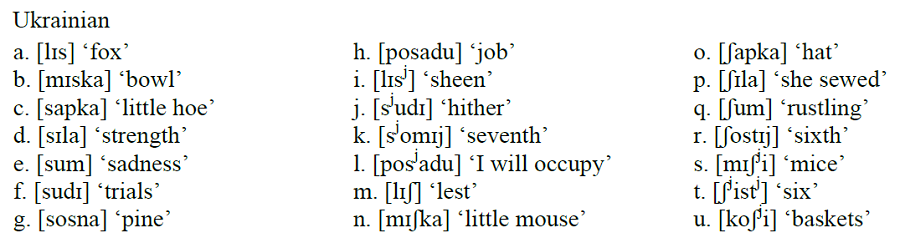
\includegraphics{../images/ukrainian.png}
\end{figure}

~\\
INSTRUCTOR NOTES: 


\vfill
Excellent (3) ~~~ Good (2.2) ~~~ Fair (1.7) ~~~ Poor (0)
\newpage

{\large Question 2}\\

Source: Day 2 Handout\\

Is this a reasonable transcription of this word? Explain why.\\

<mouse>: {[mɔɪs]}


~\\
INSTRUCTOR NOTES: no, [ɑʊ]


\vfill
Excellent (3) ~~~ Good (2.2) ~~~ Fair (1.7) ~~~ Poor (0)
\newpage

{\large Question 3}\\

Source: Day 2 Handout, Part II, Question 9\\

Explain how to figure out what the sound being produced is in this diagram.\\

\begin{figure}[H]
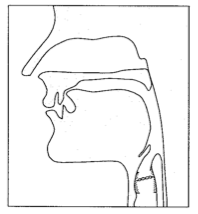
\includegraphics{../images/sagittal_z.png}
\end{figure}

~\\
INSTRUCTOR NOTES: [z] (check voicing, place, manner, and velum)


\vfill
Excellent (3) ~~~ Good (2.2) ~~~ Fair (1.7) ~~~ Poor (0)
\newpage

{\large Question 4}\\

Source: Day 7 Handout, Question 9\\

What is the basic analysis of vowel length in this dataset, and what are the key pieces of evidence?\\

\begin{figure}[H]
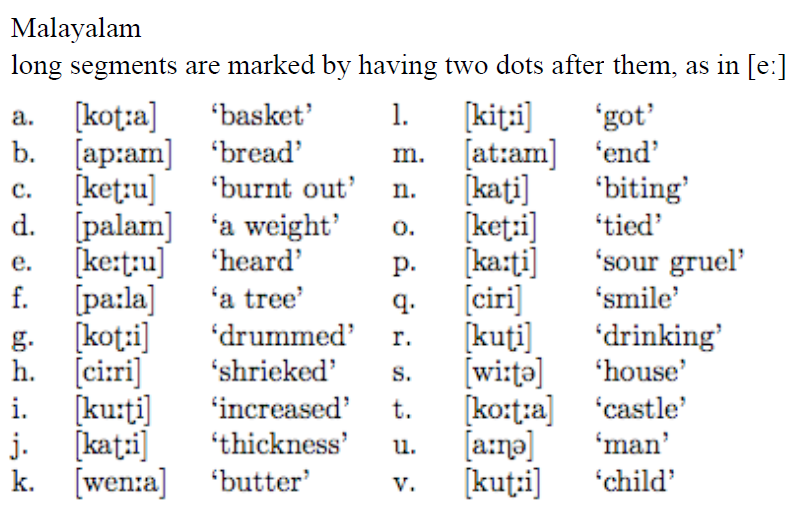
\includegraphics{../images/malayalam.png}
\end{figure}

~\\
INSTRUCTOR NOTES: Short and long vowels appear to be contrastive (phonemic) in Malayalam, as evidenced by minimal pairs that differ only in terms of their vowel length, such as [koʈːa] ‘basket’ vs. [koːʈːa] ‘castle’ or [keʈːu] ‘burnt out’ vs. [keːʈːu] ‘heard.’


\vfill
Excellent (3) ~~~ Good (2.2) ~~~ Fair (1.7) ~~~ Poor (0)
\newpage

{\large Question 5}\\

Source: Day 2 Handout, Part I, Question 2\\

Explain why people might legitimately disagree about how many sounds this particular word contains.\\

<they>


~\\
INSTRUCTOR NOTES: 


\vfill
Excellent (3) ~~~ Good (2.2) ~~~ Fair (1.7) ~~~ Poor (0)
\newpage

\begin{center}
\textbf{{\color{red}{\HUGE END OF EXAM}}}\\

\end{center}
\newpage

\begin{center}
\textbf{{\color{blue}{\HUGE START OF EXAM\\}}}

\textbf{{\color{blue}{\HUGE Student ID: 8742\\}}}

\textbf{{\color{blue}{\HUGE 3:00 - 3:15 PM\\}}}

\end{center}
\newpage

{\large Question 1}\\

Source: Quiz 3, Question 1\\

L$_X$ (Language X) has three vowels, [i], [a], and [u]. It has bi-syllabic roots like Kikuyu. It does not allow non-identical high vowels to co-occur. Of the following nine logically possible vocalic sequences, which ones should be unattested in L$_X$? Explain why.\\

\begin{itemize} \item {[i...i]} \item {[i...a]} \item {[i...u]} \item {[a...i]} \item {[a...a]} \item {[a...u]} \item {[u...i]} \item {[u...a]} \item {[u...u]} \end{itemize}


~\\
INSTRUCTOR NOTES: [i...u], [u...i]


\vfill
Excellent (3) ~~~ Good (2.2) ~~~ Fair (1.7) ~~~ Poor (0)
\newpage

{\large Question 2}\\

Source: Day 2 Handout, Part I, Question 11\\

How would this word be transcribed?\\ Follow-up question: Why did you use symbol [X] instead of symbol [Y]?\\

<square>


~\\
INSTRUCTOR NOTES: [skweɪɹ]


\vfill
Excellent (3) ~~~ Good (2.2) ~~~ Fair (1.7) ~~~ Poor (0)
\newpage

{\large Question 3}\\

Source: Day 6 Handout, Question 11\\

What do the two signs below tell you about the phonological status of \underline{handshape} in ASL, and why?\\

\begin{figure}[H]
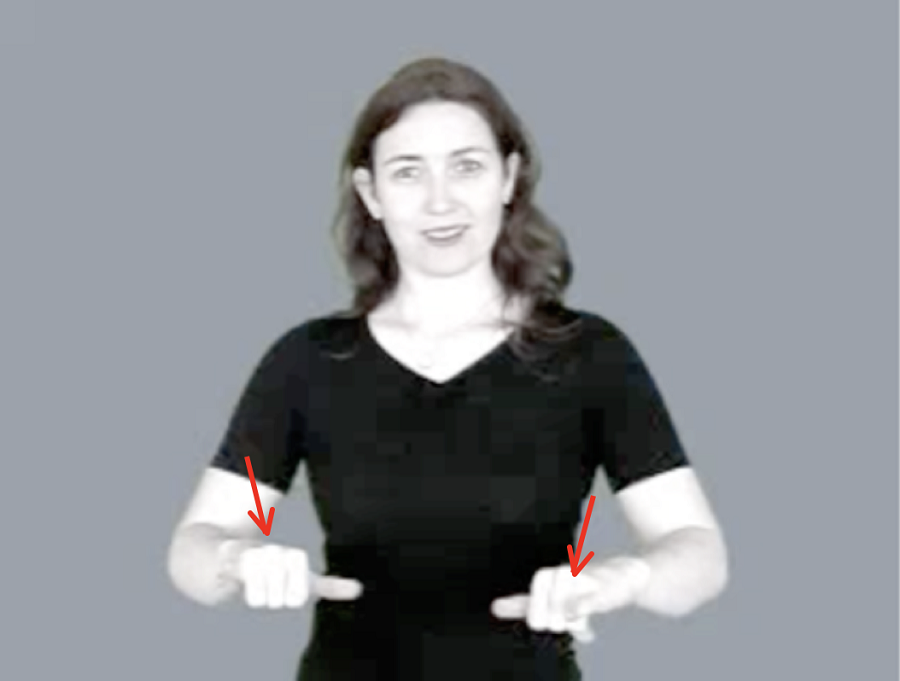
\includegraphics{../images/asl_stay.png}
\caption{STAY}
\end{figure}
\begin{figure}[H]
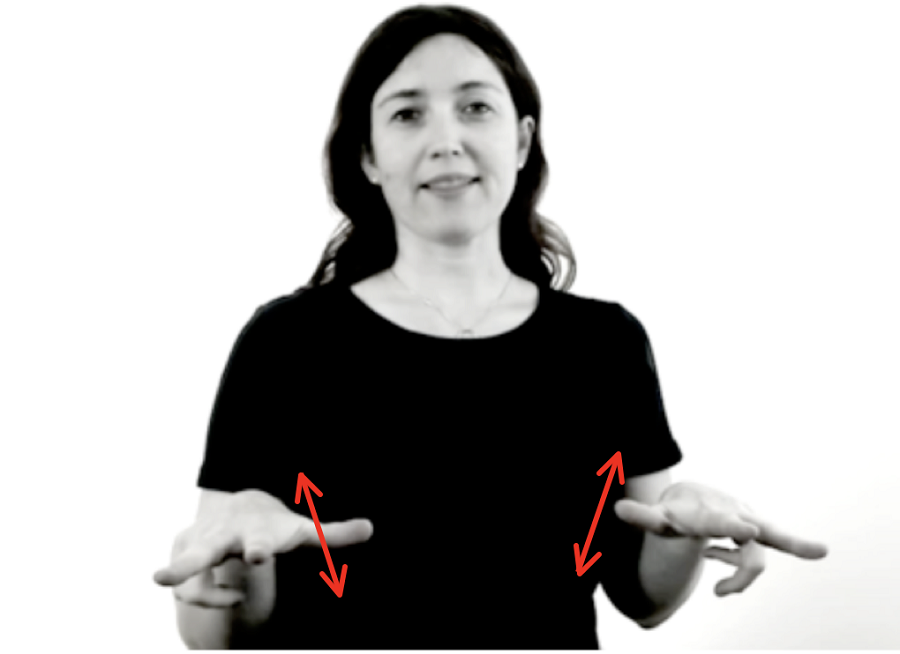
\includegraphics{../images/asl_awkward.png}
\caption{AWKWARD}
\end{figure}

~\\
INSTRUCTOR NOTES: nothing, because both handshape and movement are different


\vfill
Excellent (3) ~~~ Good (2.2) ~~~ Fair (1.7) ~~~ Poor (0)
\newpage

{\large Question 4}\\

Source: Homework 1, Question 3(b)\\

Explain why this is or is not a complete natural class in standard North American English.\\

{[f]}, {[s]}, {[ʃ]}


~\\
INSTRUCTOR NOTES: no; voiceless fricatives include [θ], [h]


\vfill
Excellent (3) ~~~ Good (2.2) ~~~ Fair (1.7) ~~~ Poor (0)
\newpage

{\large Question 5}\\

Source: Quiz 2, Question 6\\

In the pronunciation of this word, which sounds are obstruents and which are sonorants?\\

<fricative>


~\\
INSTRUCTOR NOTES: [fɹɪkətɪv] -- sonorants: [ɹɪəɪ] and obstruents: [fktv]


\vfill
Excellent (3) ~~~ Good (2.2) ~~~ Fair (1.7) ~~~ Poor (0)
\newpage

\begin{center}
\textbf{{\color{red}{\HUGE END OF EXAM}}}\\

\end{center}
\newpage

\begin{center}
\textbf{{\color{blue}{\HUGE START OF EXAM\\}}}

\textbf{{\color{blue}{\HUGE Student ID: 4199\\}}}

\textbf{{\color{blue}{\HUGE 3:15 - 3:30 PM\\}}}

\end{center}
\newpage

{\large Question 1}\\

Source: Quiz 3, Question 1\\

L$_X$ (Language X) has three vowels, [i], [a], and [u]. It has bi-syllabic roots like Kikuyu. It does not allow non-identical high vowels to co-occur. Of the following nine logically possible vocalic sequences, which ones should be unattested in L$_X$? Explain why.\\

\begin{itemize} \item {[i...i]} \item {[i...a]} \item {[i...u]} \item {[a...i]} \item {[a...a]} \item {[a...u]} \item {[u...i]} \item {[u...a]} \item {[u...u]} \end{itemize}


~\\
INSTRUCTOR NOTES: [i...u], [u...i]


\vfill
Excellent (3) ~~~ Good (2.2) ~~~ Fair (1.7) ~~~ Poor (0)
\newpage

{\large Question 2}\\

Source: Day 2 Handout, Part I, Question 11\\

How would this word be transcribed?\\ Follow-up question: Why did you use symbol [X] instead of symbol [Y]?\\

<nice>


~\\
INSTRUCTOR NOTES: [nɑɪs]


\vfill
Excellent (3) ~~~ Good (2.2) ~~~ Fair (1.7) ~~~ Poor (0)
\newpage

{\large Question 3}\\

Source: Homework 2, Question 1\\

What would this Klingon phrase below be in English? How do you know?\\

{[pɑdɑq]}

\begin{figure}[H]
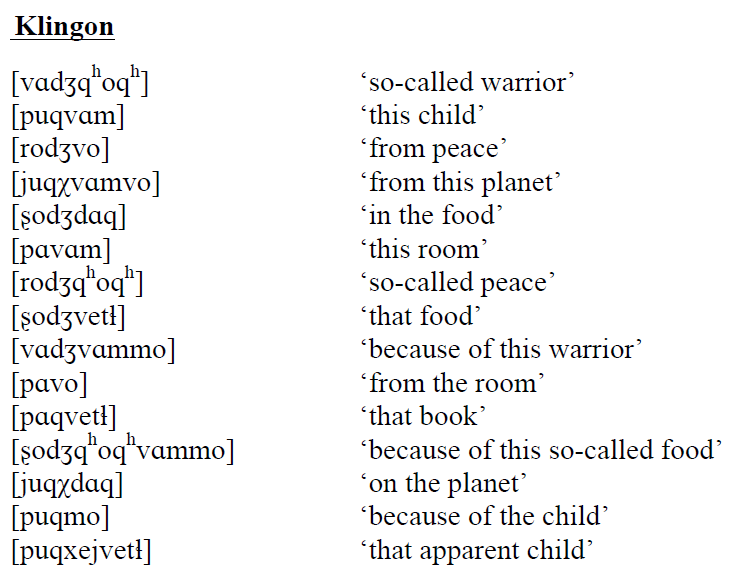
\includegraphics{../images/klingon.png}
\end{figure}

~\\
INSTRUCTOR NOTES: ‘in/on (the) room’


\vfill
Excellent (3) ~~~ Good (2.2) ~~~ Fair (1.7) ~~~ Poor (0)
\newpage

{\large Question 4}\\

Source: Day 2 Discussion\\

Assuming a Standard North American English inventory, does this vowel need to have tenseness specified if you're giving a prose description? Why or why not?\\

{[ɛ]}


~\\
INSTRUCTOR NOTES: yes


\vfill
Excellent (3) ~~~ Good (2.2) ~~~ Fair (1.7) ~~~ Poor (0)
\newpage

{\large Question 5}\\

Source: Day 6 Handout, Question 11\\

What do the two signs below tell you about the phonological status of \underline{handshape} in ASL, and why?\\

\begin{figure}[H]
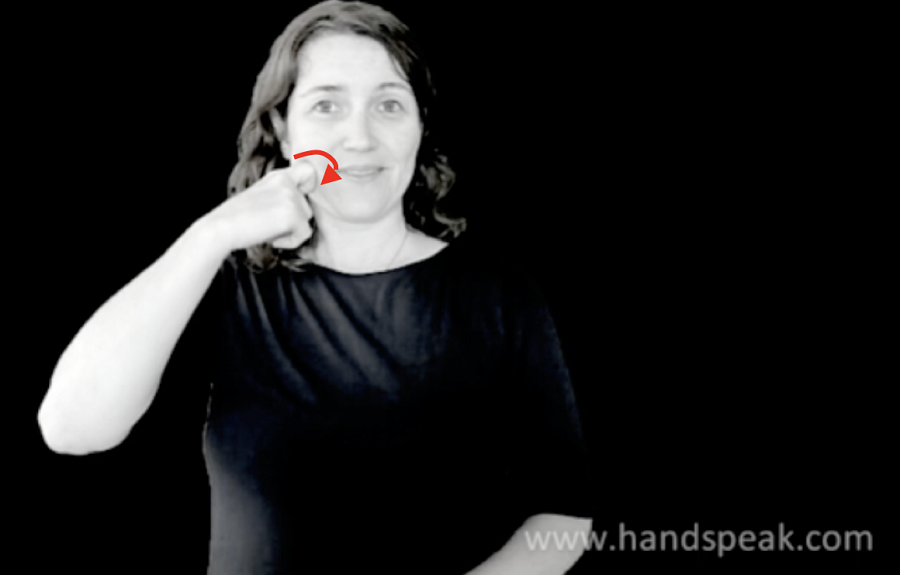
\includegraphics{../images/asl_apple.png}
\caption{APPLE}
\end{figure}
\begin{figure}[H]
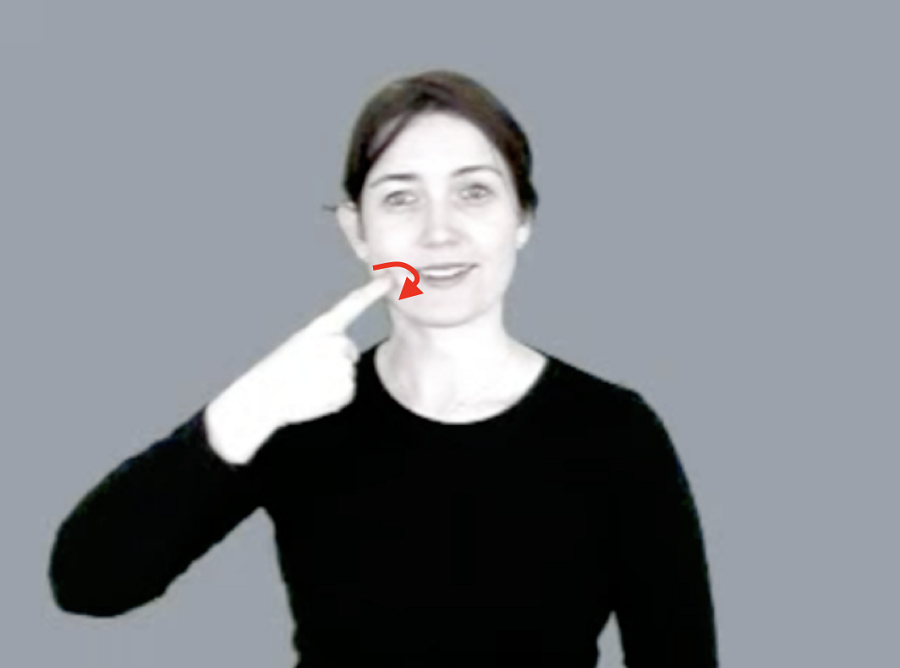
\includegraphics{../images/asl_candy.png}
\caption{CANDY}
\end{figure}

~\\
INSTRUCTOR NOTES: shows contrast because movement and location are same


\vfill
Excellent (3) ~~~ Good (2.2) ~~~ Fair (1.7) ~~~ Poor (0)
\newpage

\begin{center}
\textbf{{\color{red}{\HUGE END OF EXAM}}}\\

\end{center}
\newpage

\begin{center}
\textbf{{\color{blue}{\HUGE START OF EXAM\\}}}

\textbf{{\color{blue}{\HUGE Student ID: 3514\\}}}

\textbf{{\color{blue}{\HUGE 3:30 - 3:45 PM\\}}}

\end{center}
\newpage

{\large Question 1}\\

Source: Quiz 3, Question 1\\

L$_X$ (Language X) has three vowels, [i], [a], and [u]. It has bi-syllabic roots like Kikuyu. It does not allow non-identical high vowels to co-occur. Of the following nine logically possible vocalic sequences, which ones should be unattested in L$_X$? Explain why.\\

\begin{itemize} \item {[i...i]} \item {[i...a]} \item {[i...u]} \item {[a...i]} \item {[a...a]} \item {[a...u]} \item {[u...i]} \item {[u...a]} \item {[u...u]} \end{itemize}


~\\
INSTRUCTOR NOTES: [i...u], [u...i]


\vfill
Excellent (3) ~~~ Good (2.2) ~~~ Fair (1.7) ~~~ Poor (0)
\newpage

{\large Question 2}\\

Source: Day 6 Handout, Question 5\\

Is the statement given below a good description of the distribution of sounds in this dataset? Why or why not?\\

The sounds {[pʰ]} and {[p̚]} are in complementary distribution. {[pʰ]} occurs after front vowels, as in {[kæpʰ]} ‘cap,’ while {[p̚]} occurs after back vowels, as in {[tʃɑp̚]} ‘chop.’

\begin{figure}[H]
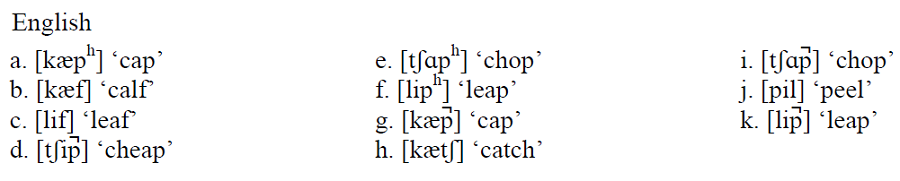
\includegraphics{../images/english_labials.png}
\end{figure}

~\\
INSTRUCTOR NOTES: no; the sounds are in free variation, because they can be variants of the same word, even though the example given doesn't show this


\vfill
Excellent (3) ~~~ Good (2.2) ~~~ Fair (1.7) ~~~ Poor (0)
\newpage

{\large Question 3}\\

Source: Day 6 Handout, Question 11\\

What do the two signs below tell you about the phonological status of \underline{handshape} in ASL, and why?\\

\begin{figure}[H]
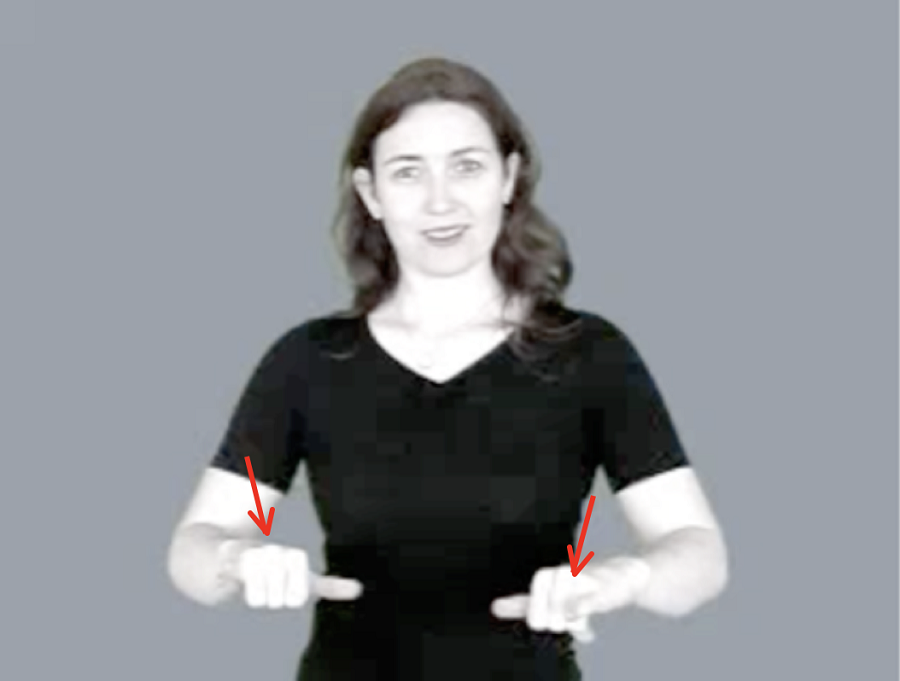
\includegraphics{../images/asl_stay.png}
\caption{STAY}
\end{figure}
\begin{figure}[H]
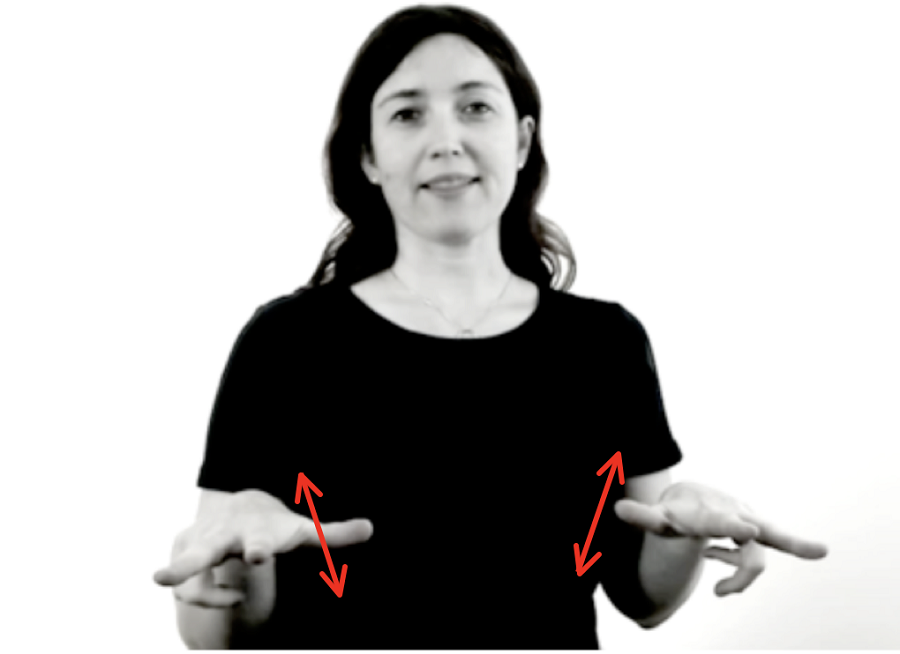
\includegraphics{../images/asl_awkward.png}
\caption{AWKWARD}
\end{figure}

~\\
INSTRUCTOR NOTES: nothing, because both handshape and movement are different


\vfill
Excellent (3) ~~~ Good (2.2) ~~~ Fair (1.7) ~~~ Poor (0)
\newpage

{\large Question 4}\\

Source: Day 2 Handout, Part I, Question 11\\

How would this word be transcribed?\\ Follow-up question: Why did you use symbol [X] instead of symbol [Y]?\\

<little>


~\\
INSTRUCTOR NOTES: [lɪɾl̩]


\vfill
Excellent (3) ~~~ Good (2.2) ~~~ Fair (1.7) ~~~ Poor (0)
\newpage

{\large Question 5}\\

Source: Day 2 Handout, Part II, Question 7\\

Is the symbol given a reasonable way to transcribe any of the sounds described below? If so, which one? If not, why not?\\

{[v]}

\begin{itemize} \item voiceless palatal affricate \item voiced velar nasal \item voiceless glottal fricative \item voiced labiodental fricative \item voiced interdental fricative \item voiced palatal fricative \end{itemize}


~\\
INSTRUCTOR NOTES: yes (voiced labiodental fricative)


\vfill
Excellent (3) ~~~ Good (2.2) ~~~ Fair (1.7) ~~~ Poor (0)
\newpage

\begin{center}
\textbf{{\color{red}{\HUGE END OF EXAM}}}\\

\end{center}
\newpage

\begin{center}
\textbf{{\color{blue}{\HUGE START OF EXAM\\}}}

\textbf{{\color{blue}{\HUGE Student ID: 8350\\}}}

\textbf{{\color{blue}{\HUGE 3:45 - 4:00 PM\\}}}

\end{center}
\newpage

{\large Question 1}\\

Source: Day 5 Handout, Question 3\\

What evidence is there that there is a pattern in these data, assuming that these are the only CV and VC sequences that occur in some language?\\

{[sa]}, {[ʃi]}, {[za]}, {[ʒi]}, {[as]}, {[iʃ]}, {[az]}, {[iʒ]}


~\\
INSTRUCTOR NOTES: (the palatal sounds occur with the high vowel, while the alveolar sounds occur with the low vowel)


\vfill
Excellent (3) ~~~ Good (2.2) ~~~ Fair (1.7) ~~~ Poor (0)
\newpage

{\large Question 2}\\

Source: Day 2 Handout, Part I, Question 11\\

How would this word be transcribed?\\ Follow-up question: Why did you use symbol [X] instead of symbol [Y]?\\

<wealth>


~\\
INSTRUCTOR NOTES: [wɛlθ]


\vfill
Excellent (3) ~~~ Good (2.2) ~~~ Fair (1.7) ~~~ Poor (0)
\newpage

{\large Question 3}\\

Source: Day 2 Handout, Part II, Question 7\\

Is the symbol given a reasonable way to transcribe any of the sounds described below? If so, which one? If not, why not?\\

{[ʃ]}

\begin{itemize} \item voiceless palatal affricate \item voiced velar nasal \item voiceless glottal fricative \item voiced labiodental fricative \item voiced interdental fricative \item voiced palatal fricative \end{itemize}


~\\
INSTRUCTOR NOTES: no (voiceless palatal fricative)


\vfill
Excellent (3) ~~~ Good (2.2) ~~~ Fair (1.7) ~~~ Poor (0)
\newpage

{\large Question 4}\\

Source: Day 2 Handout, Part II, Question 7\\

Is the symbol given a reasonable way to transcribe any of the sounds described below? If so, which one? If not, why not?\\

{[θ]}

\begin{itemize} \item voiceless palatal affricate \item voiced velar nasal \item voiceless glottal fricative \item voiced labiodental fricative \item voiced interdental fricative \item voiced palatal fricative \end{itemize}


~\\
INSTRUCTOR NOTES: no (voiceless interdental fricative)


\vfill
Excellent (3) ~~~ Good (2.2) ~~~ Fair (1.7) ~~~ Poor (0)
\newpage

{\large Question 5}\\

Source: Day 6 Handout, Question 11\\

What do the two signs below tell you about the phonological status of \underline{handshape} in ASL, and why?\\

\begin{figure}[H]
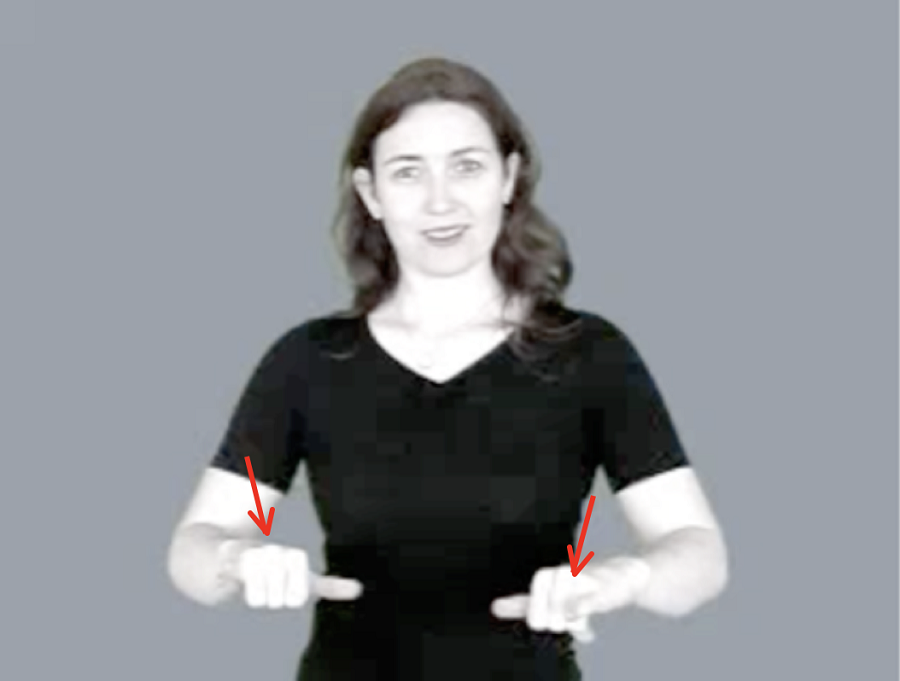
\includegraphics{../images/asl_stay.png}
\caption{STAY}
\end{figure}
\begin{figure}[H]
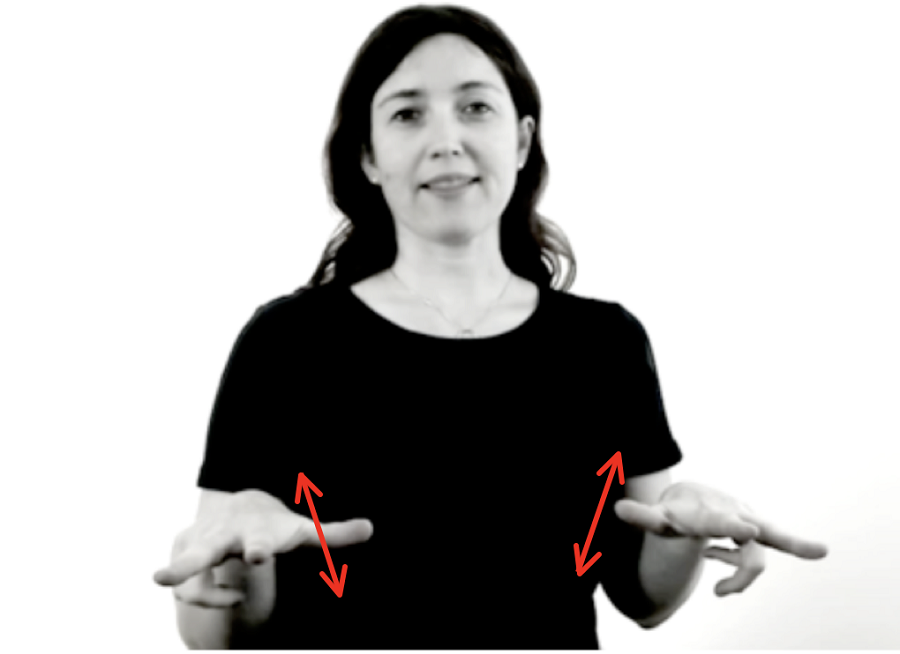
\includegraphics{../images/asl_awkward.png}
\caption{AWKWARD}
\end{figure}

~\\
INSTRUCTOR NOTES: nothing, because both handshape and movement are different


\vfill
Excellent (3) ~~~ Good (2.2) ~~~ Fair (1.7) ~~~ Poor (0)
\newpage

\begin{center}
\textbf{{\color{red}{\HUGE END OF EXAM}}}\\

\end{center}
\newpage

\begin{center}
\textbf{{\color{blue}{\HUGE START OF EXAM\\}}}

\textbf{{\color{blue}{\HUGE Student ID: 4090\\}}}

\textbf{{\color{blue}{\HUGE 4:00 - 4:15 PM\\}}}

\end{center}
\newpage

{\large Question 1}\\

Source: Quiz 3, Question 1\\

L$_X$ (Language X) has three vowels, [i], [a], and [u]. It has bi-syllabic roots like Kikuyu. It does not allow non-identical high vowels to co-occur. Of the following nine logically possible vocalic sequences, which ones should be unattested in L$_X$? Explain why.\\

\begin{itemize} \item {[i...i]} \item {[i...a]} \item {[i...u]} \item {[a...i]} \item {[a...a]} \item {[a...u]} \item {[u...i]} \item {[u...a]} \item {[u...u]} \end{itemize}


~\\
INSTRUCTOR NOTES: [i...u], [u...i]


\vfill
Excellent (3) ~~~ Good (2.2) ~~~ Fair (1.7) ~~~ Poor (0)
\newpage

{\large Question 2}\\

Source: Day 2 Handout, Part II, Question 9\\

Explain how to figure out what the sound being produced is in this diagram.\\

\begin{figure}[H]
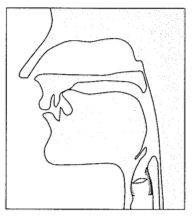
\includegraphics{../images/sagittal_t.png}
\end{figure}

~\\
INSTRUCTOR NOTES: [t] (check voicing, place, manner, and velum)


\vfill
Excellent (3) ~~~ Good (2.2) ~~~ Fair (1.7) ~~~ Poor (0)
\newpage

{\large Question 3}\\

Source: Homework 2, Question 1\\

What would this Klingon phrase below be in English? How do you know?\\

{[vɑdʒqʰoqʰvɑm]}

\begin{figure}[H]
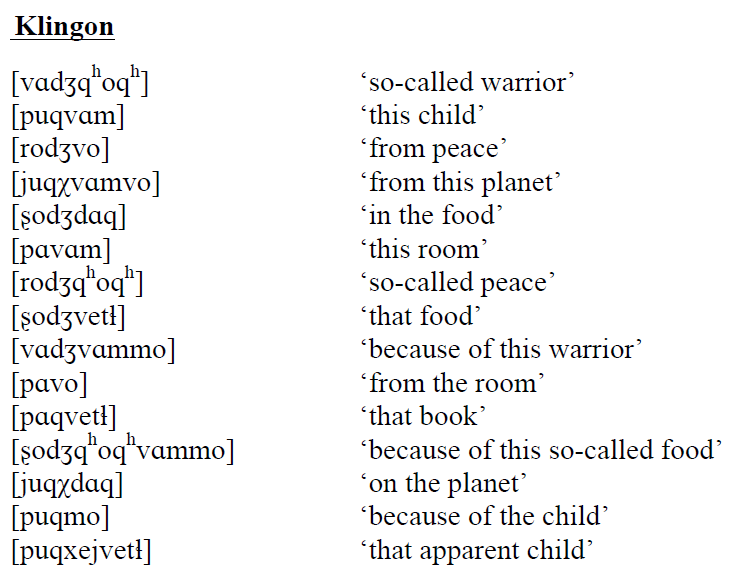
\includegraphics{../images/klingon.png}
\end{figure}

~\\
INSTRUCTOR NOTES: ‘this so-called warrior’


\vfill
Excellent (3) ~~~ Good (2.2) ~~~ Fair (1.7) ~~~ Poor (0)
\newpage

{\large Question 4}\\

Source: Day 7 Handout, Question 9\\

What is the basic analysis of vowel length in this dataset, and what are the key pieces of evidence?\\

\begin{figure}[H]
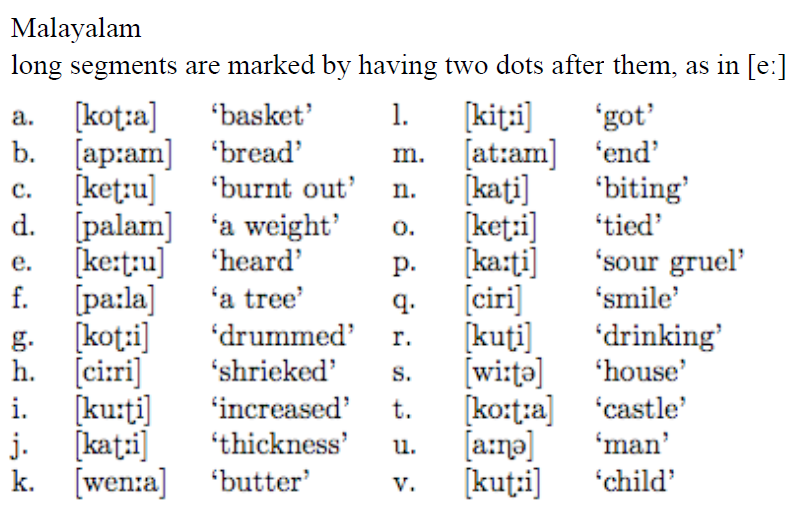
\includegraphics{../images/malayalam.png}
\end{figure}

~\\
INSTRUCTOR NOTES: Short and long vowels appear to be contrastive (phonemic) in Malayalam, as evidenced by minimal pairs that differ only in terms of their vowel length, such as [koʈːa] ‘basket’ vs. [koːʈːa] ‘castle’ or [keʈːu] ‘burnt out’ vs. [keːʈːu] ‘heard.’


\vfill
Excellent (3) ~~~ Good (2.2) ~~~ Fair (1.7) ~~~ Poor (0)
\newpage

{\large Question 5}\\

Source: Day 2 Handout, Part I, Question 11\\

How would this word be transcribed?\\ Follow-up question: Why did you use symbol [X] instead of symbol [Y]?\\

<bird>


~\\
INSTRUCTOR NOTES: [bɹ̩d]


\vfill
Excellent (3) ~~~ Good (2.2) ~~~ Fair (1.7) ~~~ Poor (0)
\newpage

\begin{center}
\textbf{{\color{red}{\HUGE END OF EXAM}}}\\

\end{center}
\newpage

\begin{center}
\textbf{{\color{blue}{\HUGE START OF EXAM\\}}}

\textbf{{\color{blue}{\HUGE Student ID: 2358\\}}}

\textbf{{\color{blue}{\HUGE 4:15 - 4:30 PM\\}}}

\end{center}
\newpage

{\large Question 1}\\

Source: Quiz 3, Question 2\\

L$_X$ has tri-syllabic roots. If L$_X$ does not allow non-identical high vowels to co-occur, which one of the following tri-syllabic vocalic sequences do you predict to be unattested in L$_X$? Explain why.\\

\begin{itemize} \item {[u...i...a]} \item {[a...i...a]} \item {[u...u...a]} \item {[a...i...i]} \end{itemize}


~\\
INSTRUCTOR NOTES: [u...i...a]


\vfill
Excellent (3) ~~~ Good (2.2) ~~~ Fair (1.7) ~~~ Poor (0)
\newpage

{\large Question 2}\\

Source: Homework 1, Question 3(b)\\

Explain why this is or is not a complete natural class in standard North American English.\\

{[b]}, {[n]}, {[ɡ]}, {[ʒ]}, {[v]}


~\\
INSTRUCTOR NOTES: no; lots of other voiced consonants


\vfill
Excellent (3) ~~~ Good (2.2) ~~~ Fair (1.7) ~~~ Poor (0)
\newpage

{\large Question 3}\\

Source: Day 2 Handout, Part I, Question 11\\

How would this word be transcribed?\\ Follow-up question: Why did you use symbol [X] instead of symbol [Y]?\\

<toy>


~\\
INSTRUCTOR NOTES: [tɔɪ]


\vfill
Excellent (3) ~~~ Good (2.2) ~~~ Fair (1.7) ~~~ Poor (0)
\newpage

{\large Question 4}\\

Source: Day 6 Handout, Question 11\\

What do the two signs below tell you about the phonological status of \underline{handshape} in ASL, and why?\\

\begin{figure}[H]
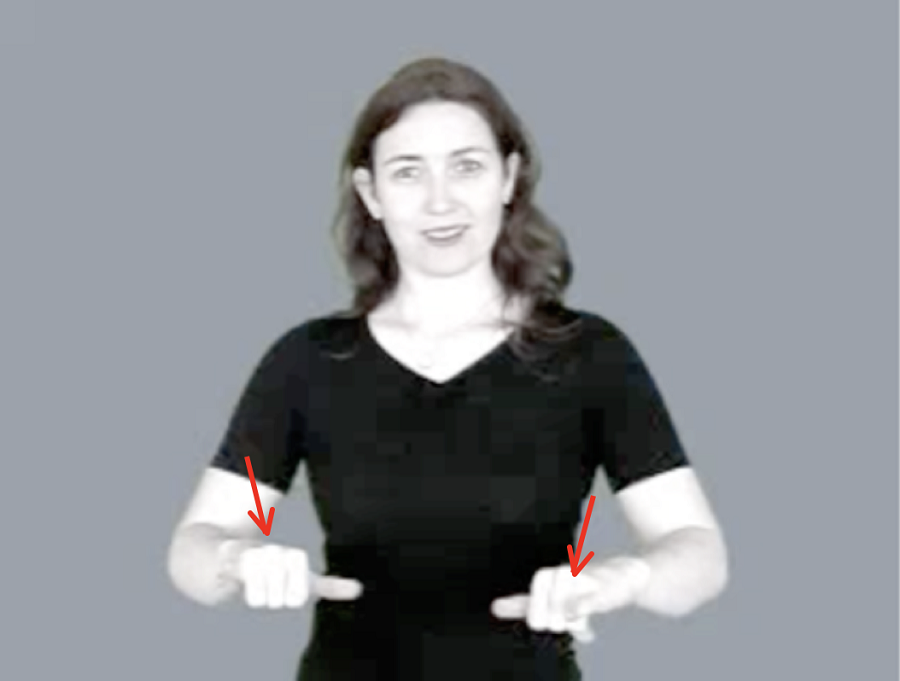
\includegraphics{../images/asl_stay.png}
\caption{STAY}
\end{figure}
\begin{figure}[H]
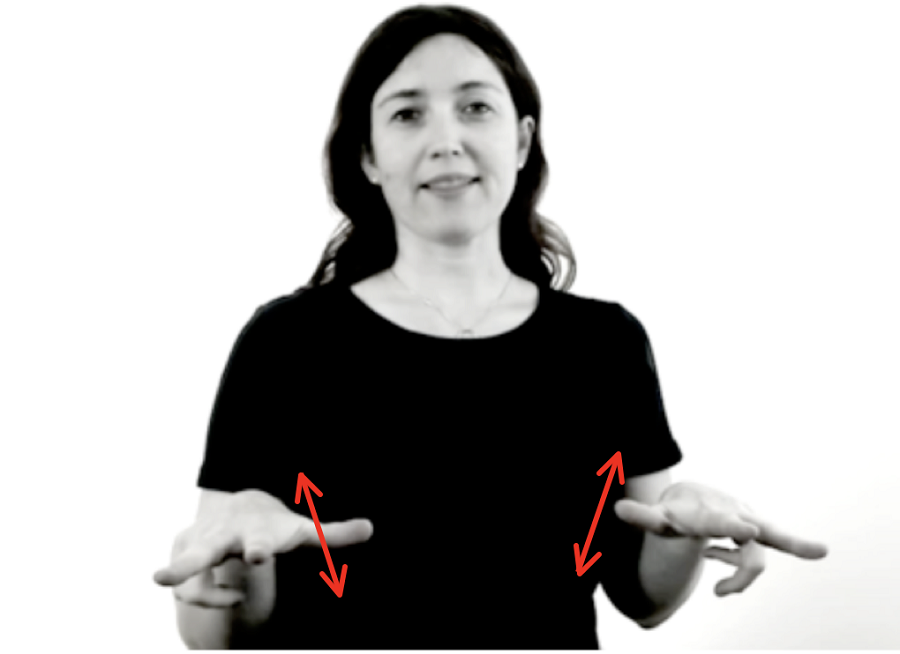
\includegraphics{../images/asl_awkward.png}
\caption{AWKWARD}
\end{figure}

~\\
INSTRUCTOR NOTES: nothing, because both handshape and movement are different


\vfill
Excellent (3) ~~~ Good (2.2) ~~~ Fair (1.7) ~~~ Poor (0)
\newpage

{\large Question 5}\\

Source: Homework 2, Question 1\\

What would this Klingon phrase below be in English? How do you know?\\

{[pɑdɑq]}

\begin{figure}[H]
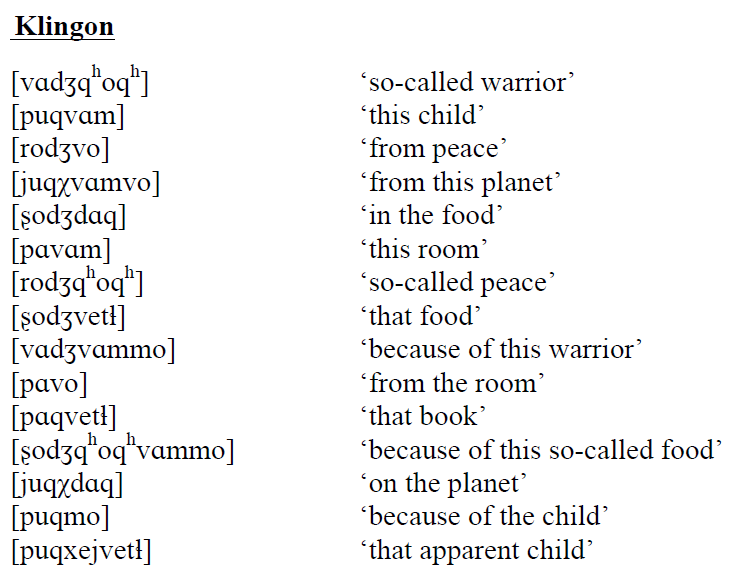
\includegraphics{../images/klingon.png}
\end{figure}

~\\
INSTRUCTOR NOTES: ‘in/on (the) room’


\vfill
Excellent (3) ~~~ Good (2.2) ~~~ Fair (1.7) ~~~ Poor (0)
\newpage

\begin{center}
\textbf{{\color{red}{\HUGE END OF EXAM}}}\\

\end{center}
\newpage

\begin{center}
\textbf{{\color{blue}{\HUGE START OF EXAM\\}}}

\textbf{{\color{blue}{\HUGE Student ID: 9376\\}}}

\textbf{{\color{blue}{\HUGE 4:30 - 4:45 PM\\}}}

\end{center}
\newpage

{\large Question 1}\\

Source: Day 5 Handout, Question 3\\

What evidence is there that there is a pattern in these data, assuming that these are the only CV and VC sequences that occur in some language?\\

{[sa]}, {[ʃi]}, {[za]}, {[ʒi]}, {[as]}, {[iʃ]}, {[az]}, {[iʒ]}


~\\
INSTRUCTOR NOTES: (the palatal sounds occur with the high vowel, while the alveolar sounds occur with the low vowel)


\vfill
Excellent (3) ~~~ Good (2.2) ~~~ Fair (1.7) ~~~ Poor (0)
\newpage

{\large Question 2}\\

Source: Day 2 Handout, Part I, Question 3\\

Explain why people might legitimately disagree about how many sounds this particular word contains.\\

<curtain>


~\\
INSTRUCTOR NOTES: 


\vfill
Excellent (3) ~~~ Good (2.2) ~~~ Fair (1.7) ~~~ Poor (0)
\newpage

{\large Question 3}\\

Source: Day 6 Handout, Question 5\\

Explain how you would determine the phonological relationship between these two sounds (given below) in this dataset.\\

{[pʰ]} and {[f]}

\begin{figure}[H]
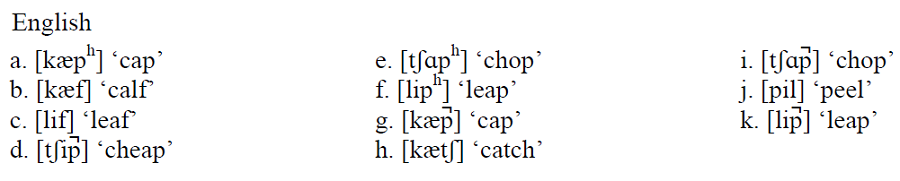
\includegraphics{../images/english_labials.png}
\end{figure}

~\\
INSTRUCTOR NOTES: contrastive; minimal pair


\vfill
Excellent (3) ~~~ Good (2.2) ~~~ Fair (1.7) ~~~ Poor (0)
\newpage

{\large Question 4}\\

Source: Homework 1, Question 3(a)\\

Could this image be the result of producing the sound represented by the given IPA symbol? Why or why not?\\

{[d]}

\begin{figure}[H]
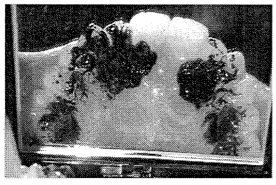
\includegraphics{../images/staticpalatography_fricative.png}
\end{figure}

~\\
INSTRUCTOR NOTES: no; space


\vfill
Excellent (3) ~~~ Good (2.2) ~~~ Fair (1.7) ~~~ Poor (0)
\newpage

{\large Question 5}\\

Source: Day 6 Handout, Question 11\\

What do the two signs below tell you about the phonological status of \underline{handshape} in ASL, and why?\\

\begin{figure}[H]
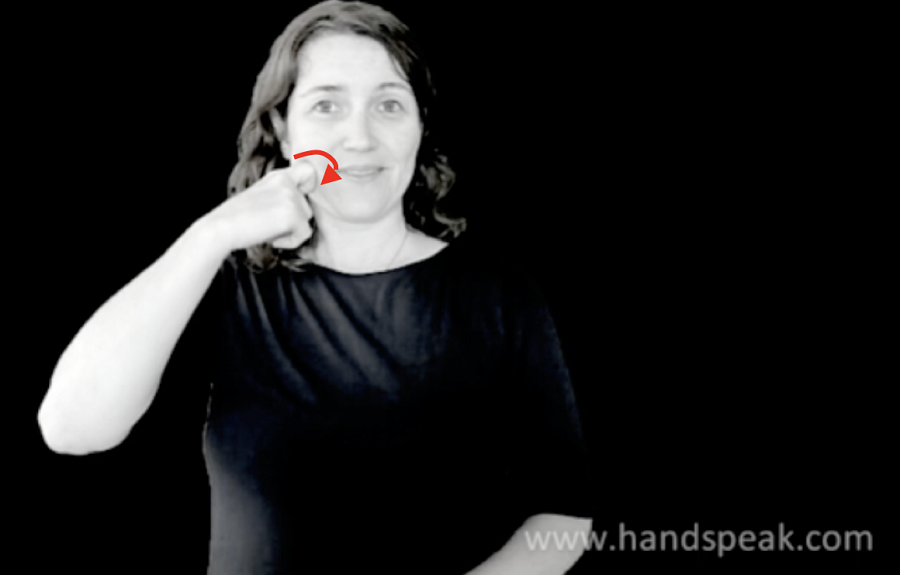
\includegraphics{../images/asl_apple.png}
\caption{APPLE}
\end{figure}
\begin{figure}[H]
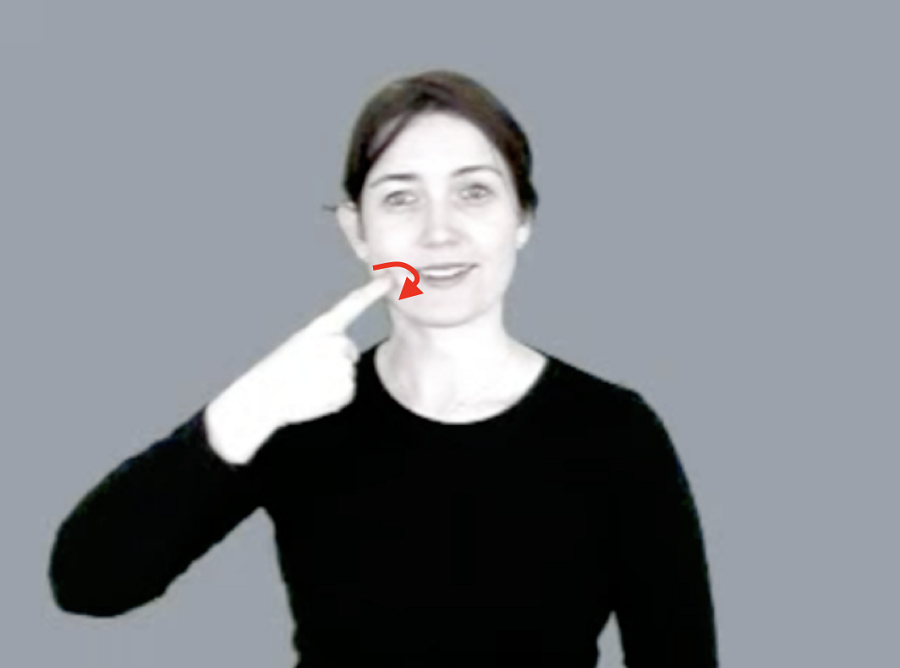
\includegraphics{../images/asl_candy.png}
\caption{CANDY}
\end{figure}

~\\
INSTRUCTOR NOTES: shows contrast because movement and location are same


\vfill
Excellent (3) ~~~ Good (2.2) ~~~ Fair (1.7) ~~~ Poor (0)
\newpage

\begin{center}
\textbf{{\color{red}{\HUGE END OF EXAM}}}\\

\end{center}
\newpage

\end{document}

